\documentclass[12pt,letterpaper,final]{article}
\usepackage[T1]{fontenc}
\usepackage[sfdefault,scaled=.9]{FiraSans}
\usepackage{newtxsf}
\usepackage[tmargin=1in,bmargin=1in,lmargin=1in,rmargin=1in]{geometry}
\usepackage[dvipsnames]{xcolor}
\usepackage{tikz}
\usepackage{array}
\usepackage{graphicx}
\usepackage{caption}
\usepackage{subcaption}
\usepackage{pifont}
\usepackage{empheq}
\usepackage{cancel}
\usepackage{amsmath,mathtools}
\usepackage{amssymb}
\usepackage{amsfonts}
\numberwithin{equation}{section}
\usepackage{bm}
\usepackage[breaklinks=true,colorlinks=true,linkcolor=purple,urlcolor=purple,citecolor=blue,%
  pdftitle={New York City Taxi Fare Prediction},
  pdfsubject={cs.LG},%
  pdfauthor={Cedric Yu}]{hyperref}
%\usepackage{filecontents}
\usepackage{dsfont}
\usepackage{soul}
\usepackage{slashed}
\usepackage{pbox}
\usepackage{float}
\usepackage[nottoc,notlot,notlof]{tocbibind}
\allowdisplaybreaks
\hbadness=10000
\hfuzz=\maxdimen
\setcounter{tocdepth}{2}
\hypersetup{pdfpagemode=UseNone}
\usepackage{listings}

\DeclarePairedDelimiter\ceil{\lceil}{\rceil}
\DeclarePairedDelimiter\floor{\lfloor}{\rfloor}

\usepackage[most]{tcolorbox}
\tcbset{myformula/.style={colback=white, %yellow!10!white,
    colframe=black, %red!50!black,
    top=5pt,bottom=5pt,left=5pt,right=5pt,
    toprule=0.5pt,bottomrule=0.5pt,leftrule=0.5pt,rightrule=0.5pt,
    boxsep=0pt,
    arc=0pt,
    outer arc=0pt,
}}

%Symbols for author emails
 \makeatletter
\def\@fnsymbol#1{\ensuremath{\ifcase#1 \or \natural\or \flat\or \sharp\or
   \quarternote\or \halfnote\or \twonotes\or \eighthnote \or \dagger\dagger
   \or \ddagger\ddagger \else\@ctrerr\fi}}
    \makeatother

\begin{document}
\renewcommand{\Im}{{\rm Im}\,}
\renewcommand{\Re}{{\rm Re}\,}
\newcommand{\diag}{{\rm diag} \, }
\newcommand{\Tr}{{\rm Tr}\,}
\newcommand{\tr}{{\rm tr}\,}
\newcommand{\C}{{\mathcal{C}}}

\title{\vspace{-2.5cm}\color{PineGreen}\textbf{New York City Taxi Fare Prediction}}
\date{} %remove date
\author{Cedric Yu\footnote{\href{mailto:cedric.yu@nyu.edu}{cedric.yu@nyu.edu}. Last updated: \today.}}
% \email{cedric.yu@nyu.edu}
%\affiliation{%
%Department of Physics, New York University New York, NY
%}%
\maketitle
\vspace{-1cm}
\begin{abstract}
We summarise our findings on the (expired) \href{https://www.kaggle.com/c/new-york-city-taxi-fare-prediction/overview}{Kaggle competition} predicting the fare amount for a taxi ride in New York City.
\end{abstract}

%Table of contents
%\begingroup
%\hypersetup{linkcolor=black}
%\hrule height 0.75pt
%\tableofcontents
%\vspace{0.8cm}
%\hrule height 0.75pt
%\endgroup

%**\vphantom{}
%\begin{align}
% A &=     \left(\int XXX       \right.\nonumber\\
%   &\qquad \left.\vphantom{\int} YYY \dots \right)
%\end{align}

%**Box for align
%\begin{empheq}[box=\fbox]{align}
%ABD & DEF\\
%&=GHI
%\end{empheq}

%Inner box with empheq for align
%\begin{empheq}[innerbox=\fbox,
%left=L\Rightarrow]{align}
%a&=b\\
%E&=mc^2 + \int_a^a x\, dx
%\end{empheq}

%**Box for align using tcolorbox; box includes equation number
%\begin{tcolorbox}[ams align,myformula]
%ABD & DEF\\
%&=GHI
%\end{tcolorbox}

%**left brace for subequations; (1.1a) and (1.1b)
%\begin{subequations}
%\begin{empheq}[left=\empheqlbrace]{align}
%s&=1\\
%o&=8
%\end{empheq}
%\end{subequations}


%**Move left the whole align with long formulas. \hspace*{-2cm}\vbox{  \begin{align} ... \end{align}}
%\hspace*{-2cm}\vbox{
%\begin{align}
%R_1(z)&\rightarrow (1-z)^{\frac{\Delta}{2}}\left(1+\mathcal{O}(1-z)\right)\frac{\Gamma(1-ik_T)\Gamma(1-\Delta)}{\Gamma(1-\frac{\Delta}{2}-ik_{\bar{w}})\Gamma(1-\frac{\Delta}{2}-ik_w)}\nonumber\\
%&\qquad\qquad+(1-z)^{\frac{2-\Delta}{2}}\left(1+\mathcal{O}(1-z)\right)\frac{\Gamma(1-ik_T)\Gamma(\Delta-1)}{\Gamma(\frac{\Delta}{2}-ik_{\bar{w}})\Gamma(\frac{\Delta}{2}-ik_w)}\\
%R_2(z)&\rightarrow (1-z)^{\frac{\Delta}{2}}\frac{\Gamma(1+ik_T)\Gamma(1-\Delta)}{\Gamma(1-\frac{\Delta}{2}+ik_{\bar{w}})\Gamma(1-\frac{\Delta}{2}+ik_w)}+(1-z)^{\frac{2-\Delta}{2}}\frac{\Gamma(1+ik_T)\Gamma(\Delta-1)}{\Gamma(\frac{\Delta}{2}+ik_{\bar{w}})\Gamma(\frac{\Delta}{2}+ik_w)}.
%\end{align}}

%** multiple lines in one equation number
%\begin{equation}
%\begin{aligned}
%I&JKL\\
%&=MN
%\end{aligned}
%\end{equation}

%** splits formulas in align
%\begin{align}
%\begin{split}
%Rs&dd\\
%&+ss
%\end{split}
%\\
%\begin{split}
%aa&dd\\
%&+ff
%\end{split}
%\end{align}

%**  trim={<left> <lower> <right> <upper>}. clip activates cropping.
%\begin{figure}[h]
%\begin{center}
%\includegraphics[trim={0 390 400 0},clip,width=0.68\linewidth,keepaspectratio]{ADM_fig.pdf}
%\caption{Wald Fig. 10.2. The shift vector $N^a$ and the lapse function $N$.}
%\end{center}
%\end{figure}

%\begin{figure}[H]
%\centering
%\begin{subfigure}{0.8\textwidth}
%  \centering
%  \includegraphics[width=.8\linewidth,keepaspectratio]{Torus_two_tubes.pdf}
%\caption{The solid.}\label{Torus_two_tubes}
%\end{subfigure}%
%\linebreak
%\begin{subfigure}{.8\textwidth}
%  \centering
%  \includegraphics[width=.8\linewidth,keepaspectratio]{torus_dome.pdf}
%  \caption{The sad.}
%  \label{torus_dome}
%\end{subfigure}
%\caption{The sss.}
%\label{Torus_two_tubes0}
%\end{figure}

%\det\nolimits^{\perp}{(\nabla^2+2-m^2)}

%\hyperref[abc]{Section \ref*{abc}}

%\section{\texorpdfstring{$AdS_3$}{AdS3} Notation}

\section{Problem Statement}
In this competition, we are tasked with predicting the fare amount (inclusive of tolls) for a taxi ride in New York City with given datasets that include pickup and dropoff locations. A naive regression using just the Euclidean distance between the pickup and dropoff points would give a root-mean-squared-error (RMSE) of around $\$5$-$\$8$. We are asked to do better, using various techniques in feature engineering and employing more sophisticated machine learning models.

First, there are a few useful numbers. The base fare of NYC taxis is \$2.50. Added to it are 50 cents per 1/5 mile when traveling above 12mph or per 60 seconds in slow traffic or when the vehicle is stopped; plus 50 cents overnight surcharge 8pm to 6am; plus \$1.00 rush hour surcharge from 4pm to 8pm on weekdays, excluding holidays. Trips between JFK airport and Manhattan have a flat rate of \$52 (plus a \$4.50 surcharge during peak hours).  The farthest driving distance within NYC is about 45 miles (between the Bronx and Staten Island), which makes the fare about \$120, modulo toll fees. But then some people travel to/from New Jersey or Long Island. 

\subsection{Datasets}
We are given the training and test datasets, which make up 5.7GB in total. The given features are:
\begin{enumerate}
\item \verb|key|: the unique id associated to each instance containing the pickup datetime
\item \verb|pickup_datetime|: timestamp value indicating when the taxi ride started
\item \verb|pickup_longitude|: float for longitude coordinate of where the taxi ride started
\item \verb|pickup_latitude|: float for latitude coordinate of where the taxi ride started
\item \verb|dropoff_longitude|: float for longitude coordinate of where the taxi ride ended
\item \verb|dropoff_latitude|: float for latitude coordinate of where the taxi ride ended
\item \verb|passenger_count|: integer indicating the number of passengers in the taxi ride
\end{enumerate}
The target is \verb|fare_amount|: float (US) dollar amount of the cost of the taxi ride.

\subsubsection*{Preliminary Observations and Processing}
The training set (\verb|train.csv|) contains $55,423,855$ instances, while the test set (\verb|test.csv|) has $9,914$ instances. 

The training set is a large dataset; we should avoid performing same tasks repeatedly when possible, and good memory management is crucial. To the end of the first point, we first parse the \verb|pickup_datetime| column of both the training and test sets, extract the \verb|year|, \verb|month|, \verb|day|, \verb|weekday|, \verb|hour| and \verb|daylight_saving| features, and save the sets as new \verb|csv| files. (The \\ 
\verb|daylight_saving| feature is Boolean-valued which refers to whether the instance occurred when daylight saving was in effect.) This procedure is performed in \verb|parse_datetime.py|. To reduce memory use, every time we read the datasets into Python, we downcast the columns to either \verb|float32|, \verb|uint8| (\verb|uint16| for \verb|year|) or \verb|bool| accordingly. The datetime-processed training set now takes up about 1.9GB of memory.

Only the training set contains \verb|NaN|, respectively 376 instances in the \verb|dropoff_longitude| and \verb|dropoff_latitude| columns. We shall see that they will be gone after we discard outliers.


\section{Exploratory Data Analysis}

We make plots in \verb|dataset_study.py|.

\subsection{Target: \texttt{fare\_amount}}
From the whole training set, we first get the following histograms for the target \verb|fare_amount|.

\begin{figure}[H]
\centering
\begin{subfigure}{0.6\textwidth}
  \centering
  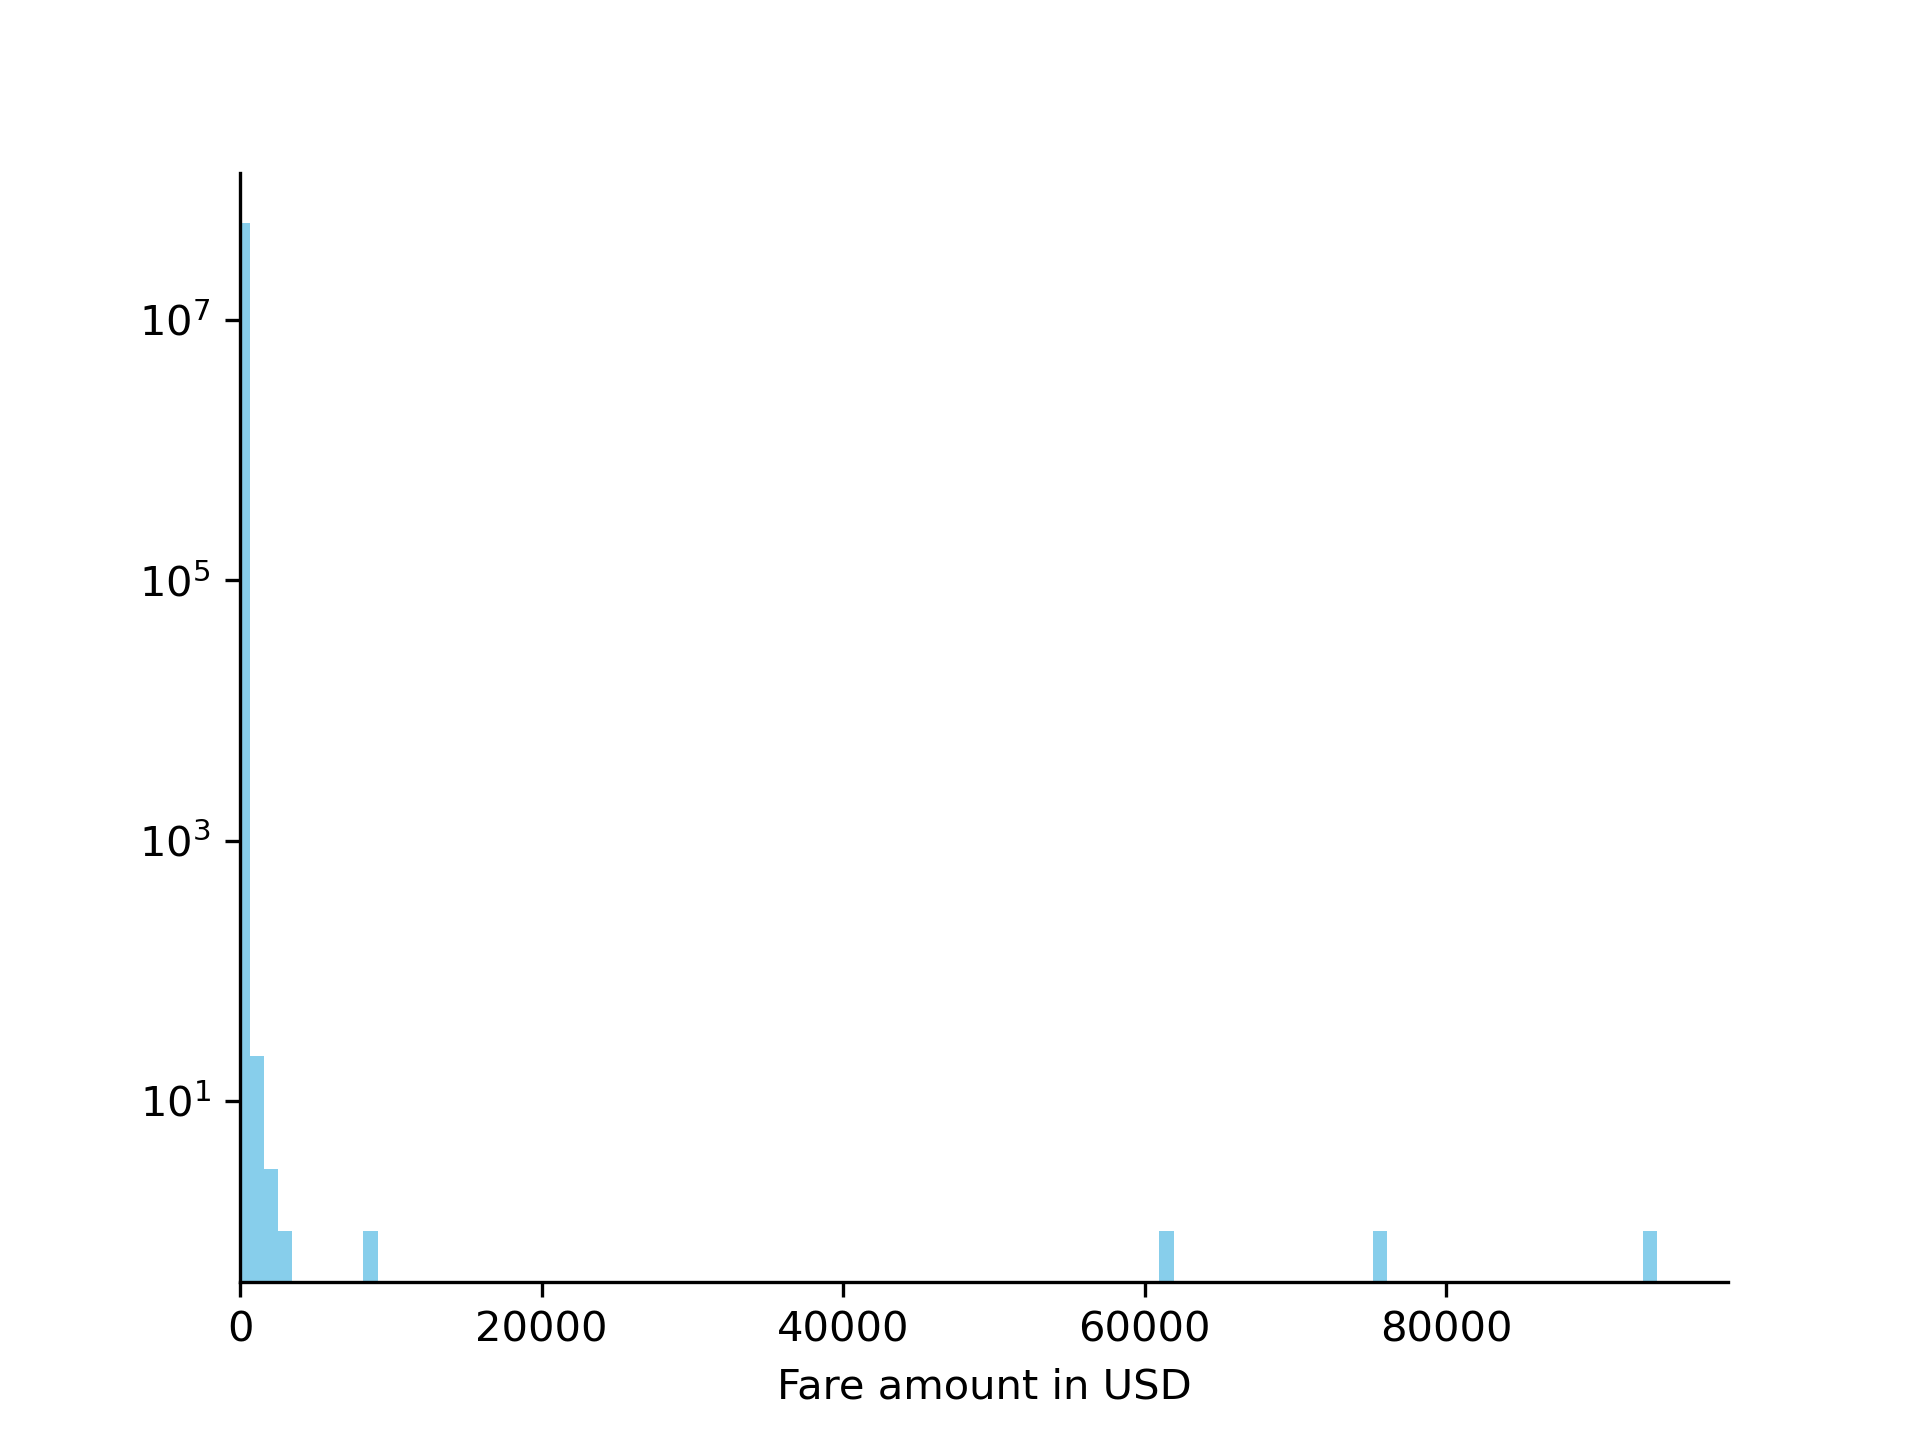
\includegraphics[width=1.\linewidth,keepaspectratio]{plots/probing_outliers/fare_amount_training_all_hist.png}
\caption{The whole range}
\end{subfigure}% 
\hspace*{-2cm}
\begin{subfigure}{.6\textwidth}
  \centering
  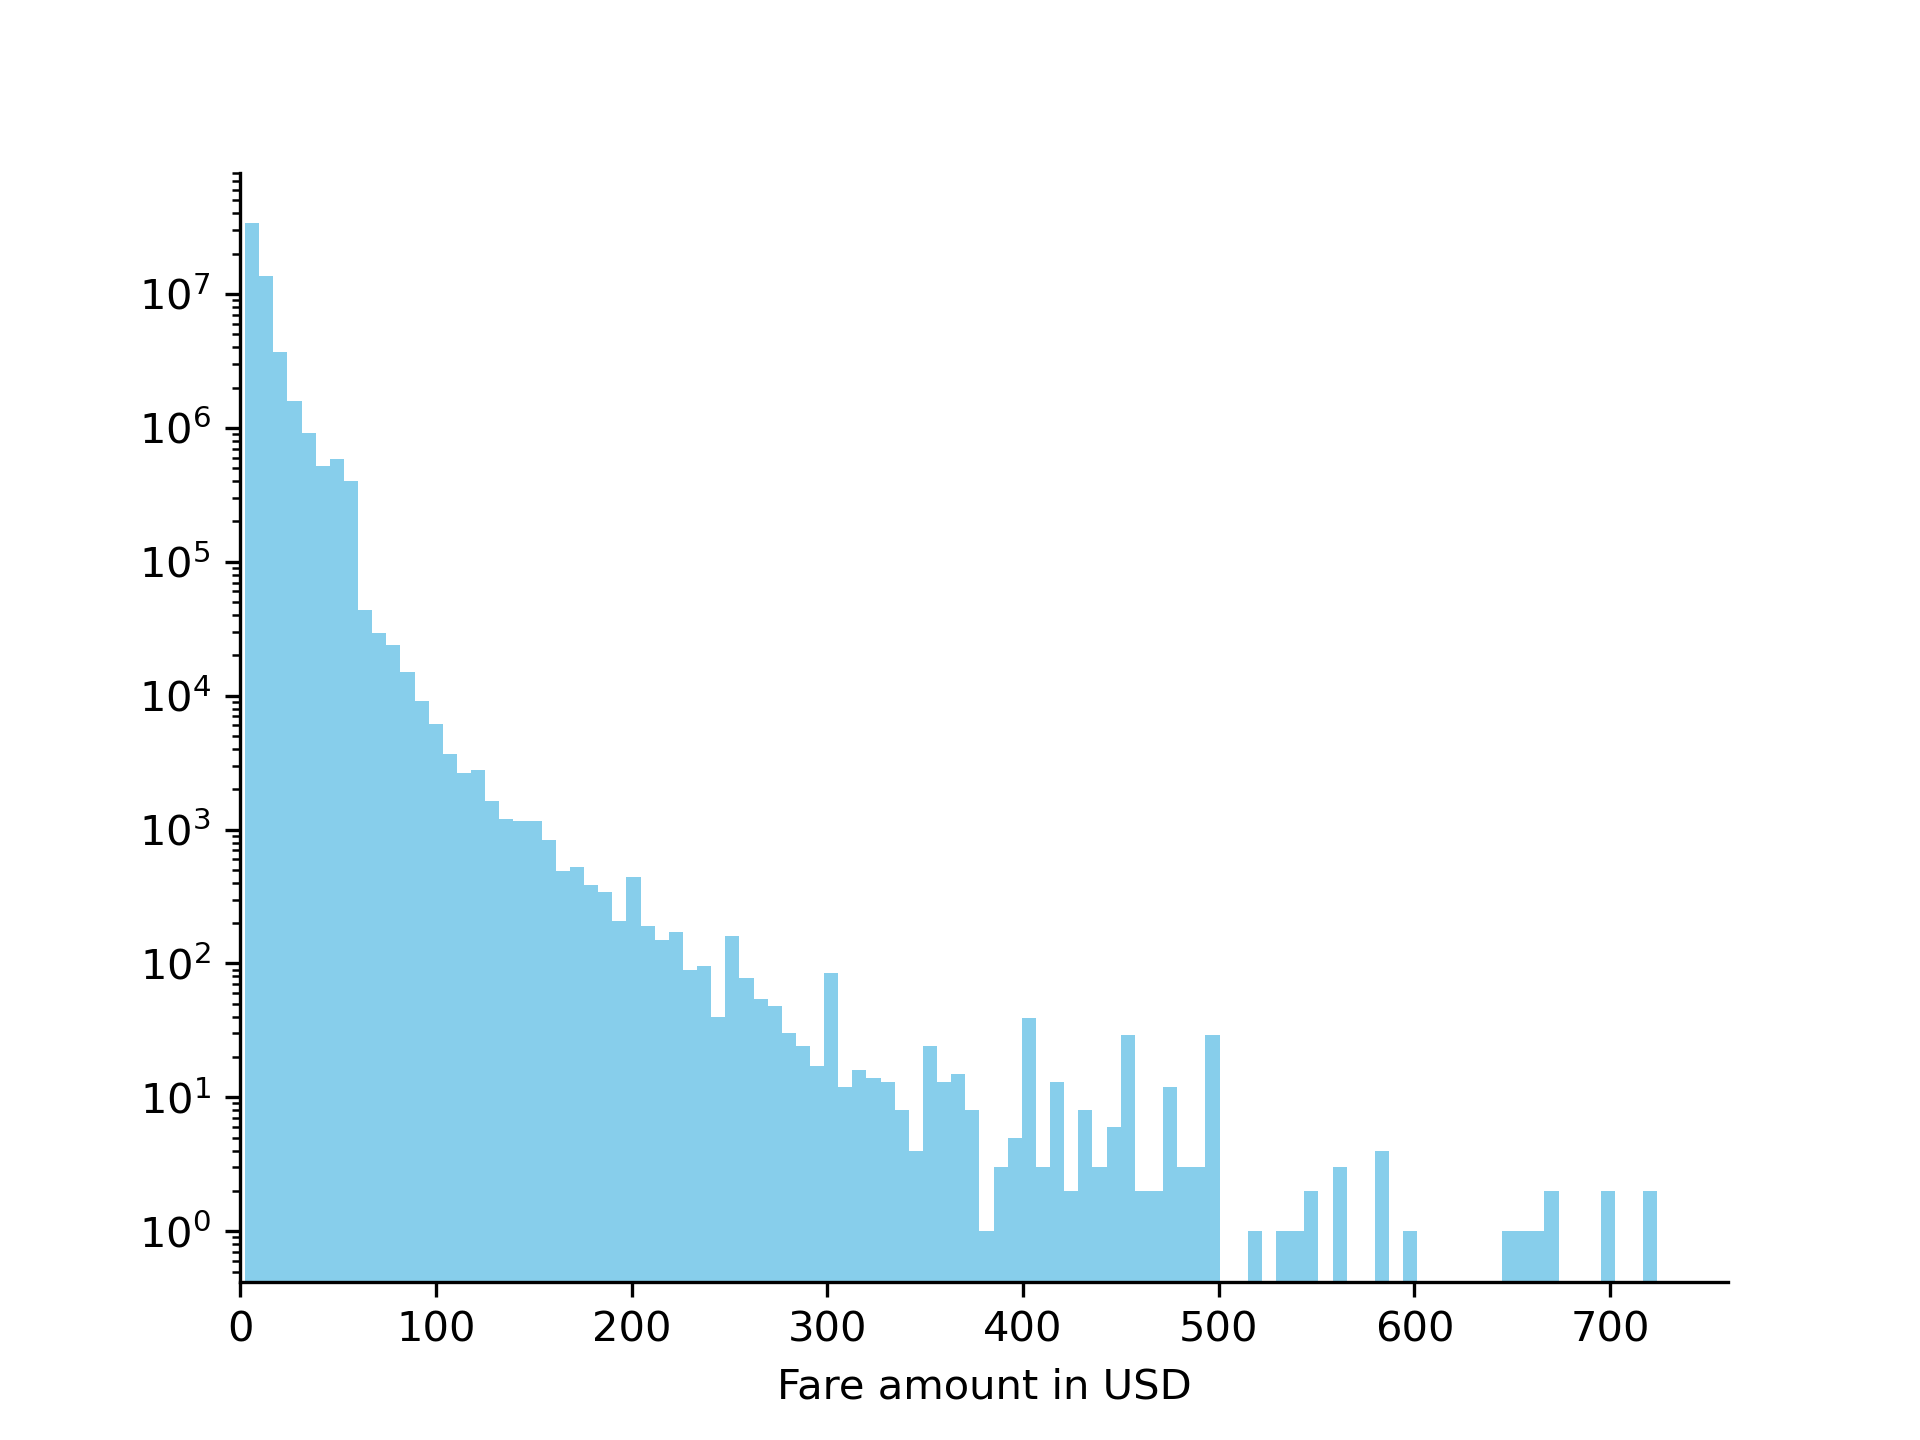
\includegraphics[width=1.\linewidth,keepaspectratio]{plots/probing_outliers/fare_amount_2.5_800_hist.png}
  \caption{Between \$2.50 (base fare) and \$800}
  \label{fare_amount_2}
\end{subfigure}
\caption{Histogram of \texttt{fare\_amount} from the whole training set, in log scale.}
\label{fare_amount_training_all_hist}
\end{figure}

Given the real-life numbers listed in the last section, any \verb|fare_amount| larger than \$1,000 does not make sense. We make a choice to only keep instances with \verb|fare_amount| between \$2.50 (base fare) and \$800 inclusive. See \hyperref[fare_amount_2]{Figure \ref*{fare_amount_2}}.

\subsection{\texttt{passenger\_count}}

We look at the feature \verb|passenger_count|. In the training set \textit{after} keeping only instances with \verb|fare_amount| between \$2.50 (base fare) and \$800, \verb|passenger_count| has the following distribution:

\vspace*{-20pt}

\begin{figure}[H]
\begin{center}
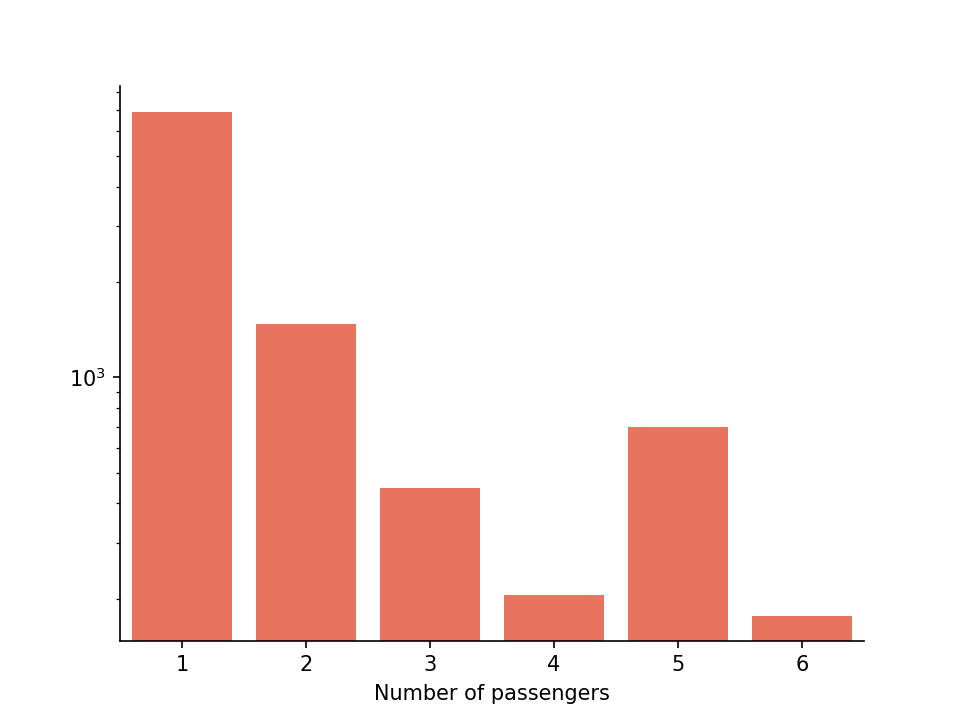
\includegraphics[width=0.6\linewidth,keepaspectratio]{plots/probing_outliers/2_passenger_count/count by number of passengers.png}
\caption{Histogram of \texttt{passenger\_count} in the training set after the first truncation.}
\end{center}
\end{figure}

\vspace*{-20pt}

Obviously, those with \verb|passenger_count| larger than ten do not make much sense. Moreover, the test set only contains \verb|passenger_count| from 1 to 6. Therefore, we only keep instances with \verb|passenger_count| between 1 and 6 inclusive. Then \verb|passenger_count| in the training and test sets take very similar distributions; see \hyperref[passengers_train_test]{Figure \ref*{passengers_train_test}}.

\begin{figure}[H]
\begin{center}
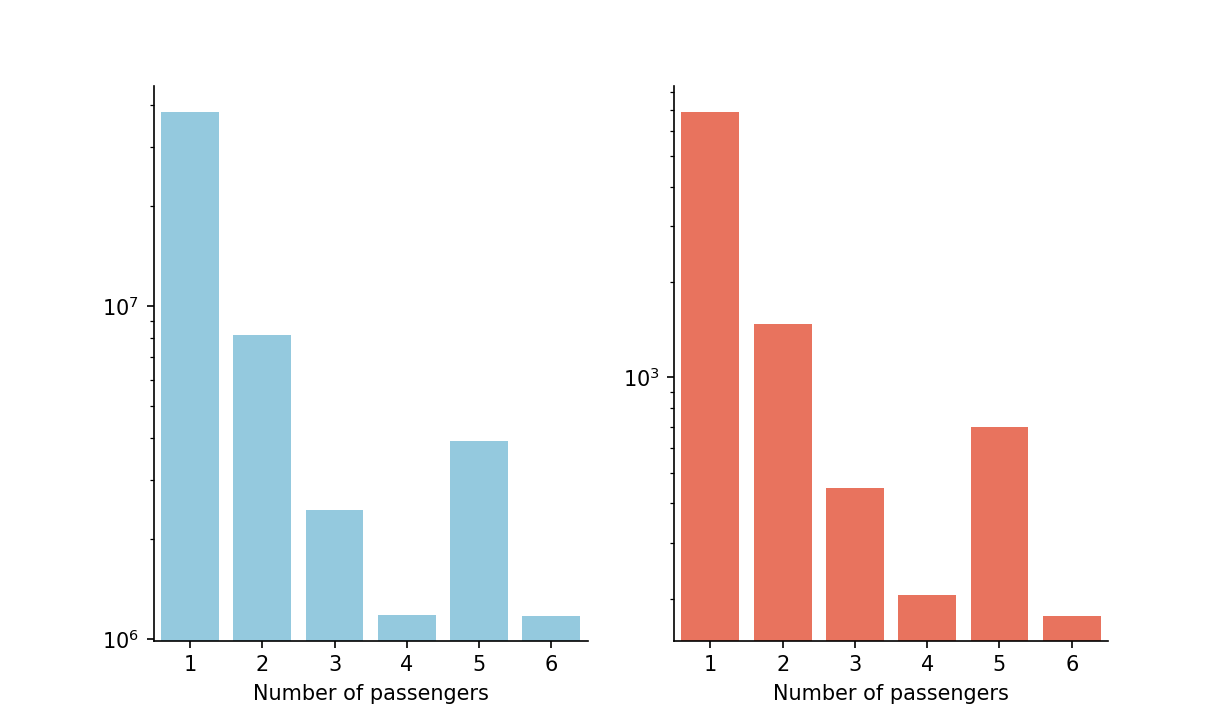
\includegraphics[width=0.8\linewidth,keepaspectratio]{plots/probing_outliers/2_passenger_count/count by number of passengers_train_test.png}
\caption{Histogram of \texttt{passenger\_count} (between 1 and 6 inclusive) in the twice-truncated training and test sets, \$2.50$\leq$ \texttt{fare\_amount} $\leq$\$800.}\label{passengers_train_test}
\end{center}
\end{figure}

\subsection{Datetime Features}
After the above two truncations (\verb|fare_amount| and \verb|passenger_count|), we look at the datetime features. Since the test test does not have data during year 2008, we discard those in the training set as well.

For \verb|year|, \verb|month|, \verb|day| and \verb|hour|, the respective means of \verb|fare_amount| show more clear variations than the number counts (see e.g. \hyperref[year_count_training]{Figure \ref*{year_count_training}} and \hyperref[hour_count_training]{Figure \ref*{hour_count_training}}). Therefore, it makes more sense to perform target (mean) encoding on these features.


\begin{figure}[H]
\centering
\begin{subfigure}{0.55\textwidth}
  \centering
  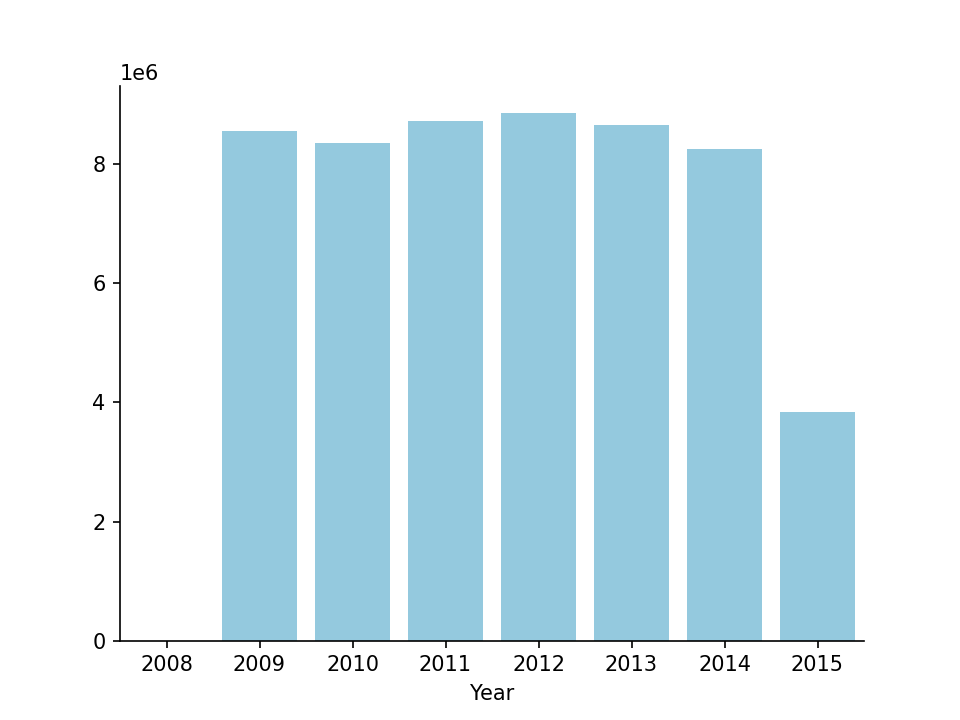
\includegraphics[width=.9\linewidth,keepaspectratio]{plots/probing_outliers/3_datetime/year_count_training.png}
\caption{Ridership count by year}
\end{subfigure}% 
\hspace*{-2cm}
\begin{subfigure}{.55\textwidth}
  \centering
  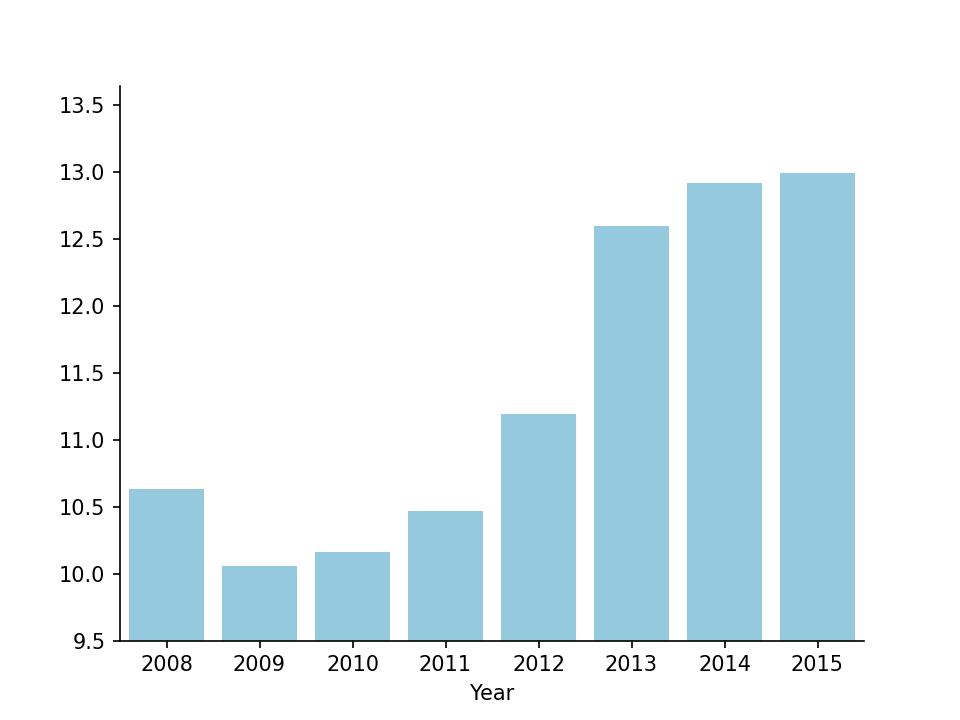
\includegraphics[width=.9\linewidth,keepaspectratio]{plots/probing_outliers/3_datetime/year_mean_fare_training.png}
  \caption{Yearly mean \texttt{fare\_amount}}
%  \label{fare_amount_2}
\end{subfigure}
\caption{Histograms of \texttt{year} feature from the twice-truncated training set.}
\label{year_count_training}
\end{figure}



\begin{figure}[H]
\centering
\begin{subfigure}{0.55\textwidth}
  \centering
  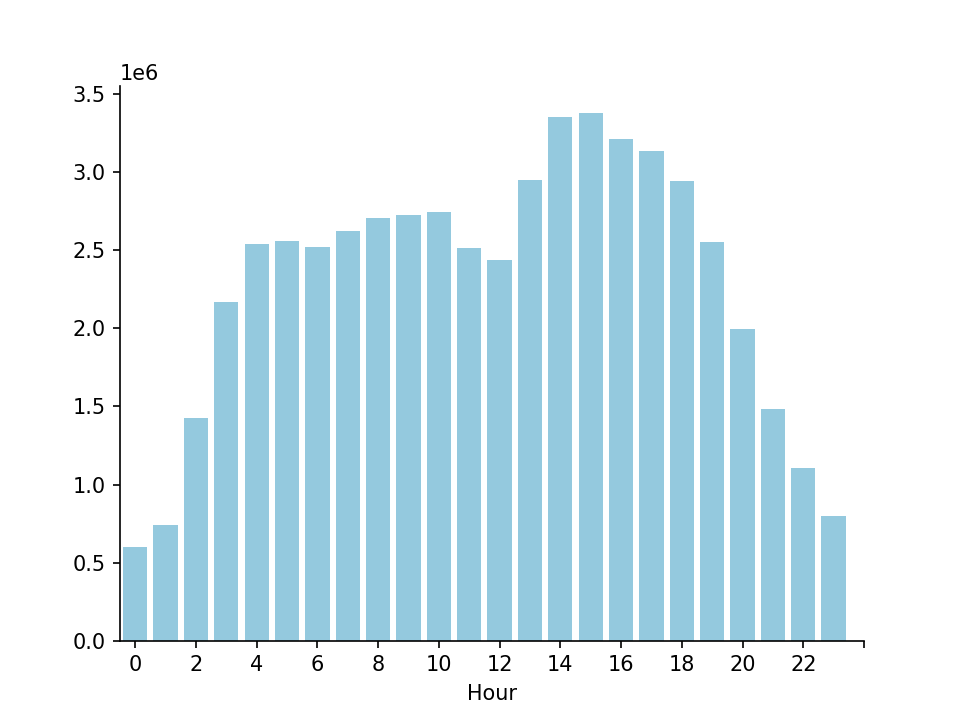
\includegraphics[width=.9\linewidth,keepaspectratio]{plots/probing_outliers/3_datetime/hour_count_training.png}
\caption{Ridership count by hour}
\end{subfigure}% 
\hspace*{-2cm}
\begin{subfigure}{.55\textwidth}
  \centering
  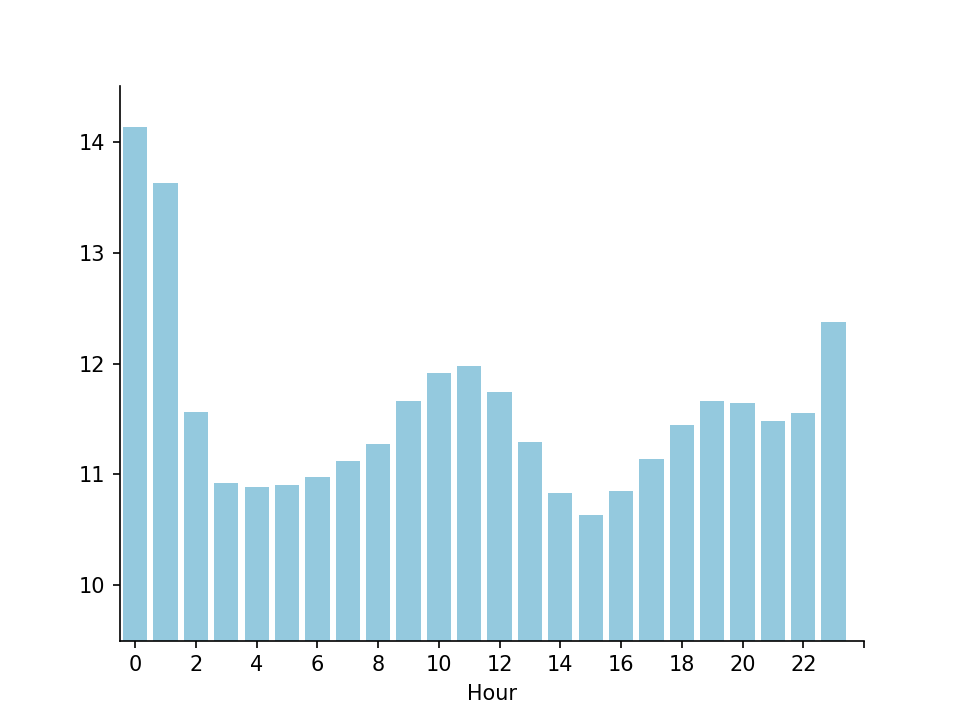
\includegraphics[width=.9\linewidth,keepaspectratio]{plots/probing_outliers/3_datetime/hour_mean_fare_training.png}
  \caption{Hourly mean \texttt{fare\_amount}}
%  \label{fare_amount_2}
\end{subfigure}
\caption{Histograms of \texttt{hour} feature from the twice-truncated training set.}
\label{hour_count_training}
\end{figure}



For \verb|weekday|, however, the frequency plot in \hyperref[weekday_count_training]{Figure \ref*{weekday_count_training}} shows a much clearer trend, so we opt to perform frequency encoding on this feature.


\begin{figure}[H]
\centering
\begin{subfigure}{0.6\textwidth}
  \centering
  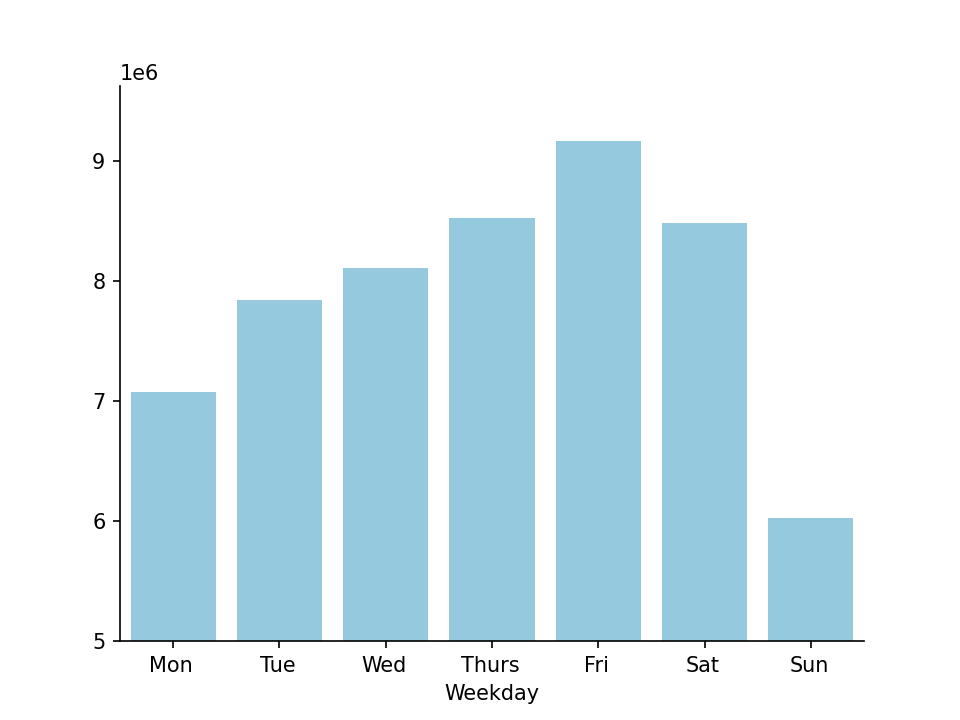
\includegraphics[width=.8\linewidth,keepaspectratio]{plots/probing_outliers/3_datetime/weekday_count_training.png}
\caption{Ridership count by weekday}
\end{subfigure}% 
\hspace*{-2cm}
\begin{subfigure}{.6\textwidth}
  \centering
  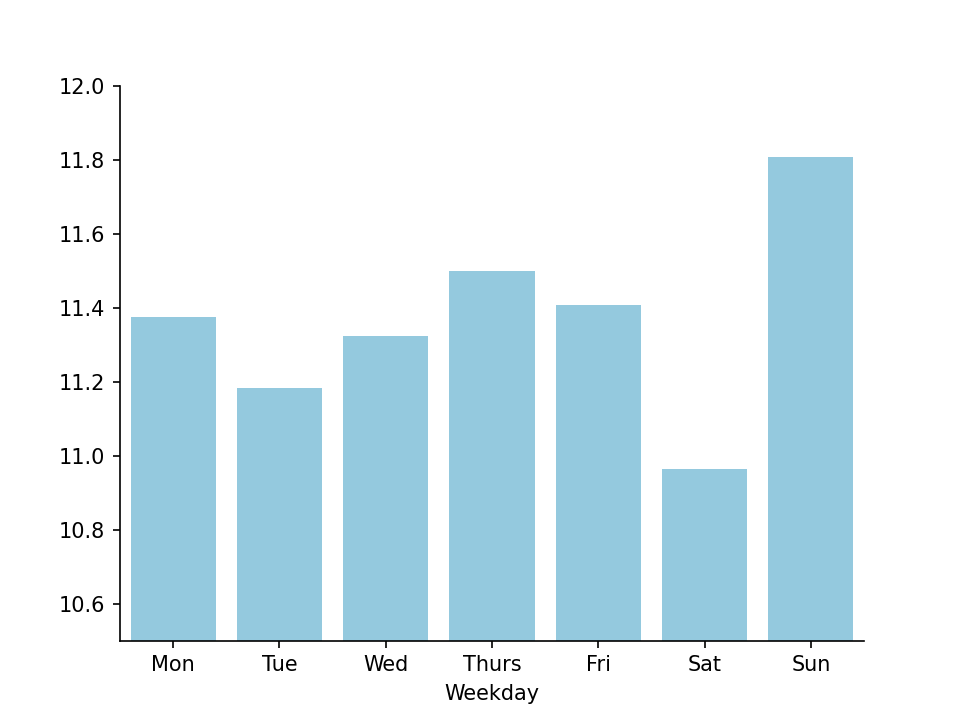
\includegraphics[width=.8\linewidth,keepaspectratio]{plots/probing_outliers/3_datetime/weekday_mean_fare_training.png}
  \caption{Mean \texttt{fare\_amount} by weekday}
%  \label{fare_amount_2}
\end{subfigure}
\caption{Histograms of \texttt{weekday} feature from the twice-truncated training set.}
\label{weekday_count_training}
\end{figure}

\subsection{Geographical Data}

At this point, we have performed three truncations (\verb|fare_amount|, \verb|passenger_count| and \verb|year|). We now explore possible truncation based on the geographical data. 

The pickup/dropoff latitudes/longitudes in the training set are as large as $\pm 3000$, and there are some with zero values. These are obviously nonsensical outliers. However, most do fall within the approximate boundary of NYC (see \hyperref[NYCmap]{Figure \ref*{NYCmap}}), whose coordinates are given by (40.40, -75.00) and (41.06, -73.33) that include some parts of New Jersey and Long Island; see \hyperref[coordinates_box]{Figure \ref*{coordinates_box}}. 


\begin{figure}[H]
\begin{center}
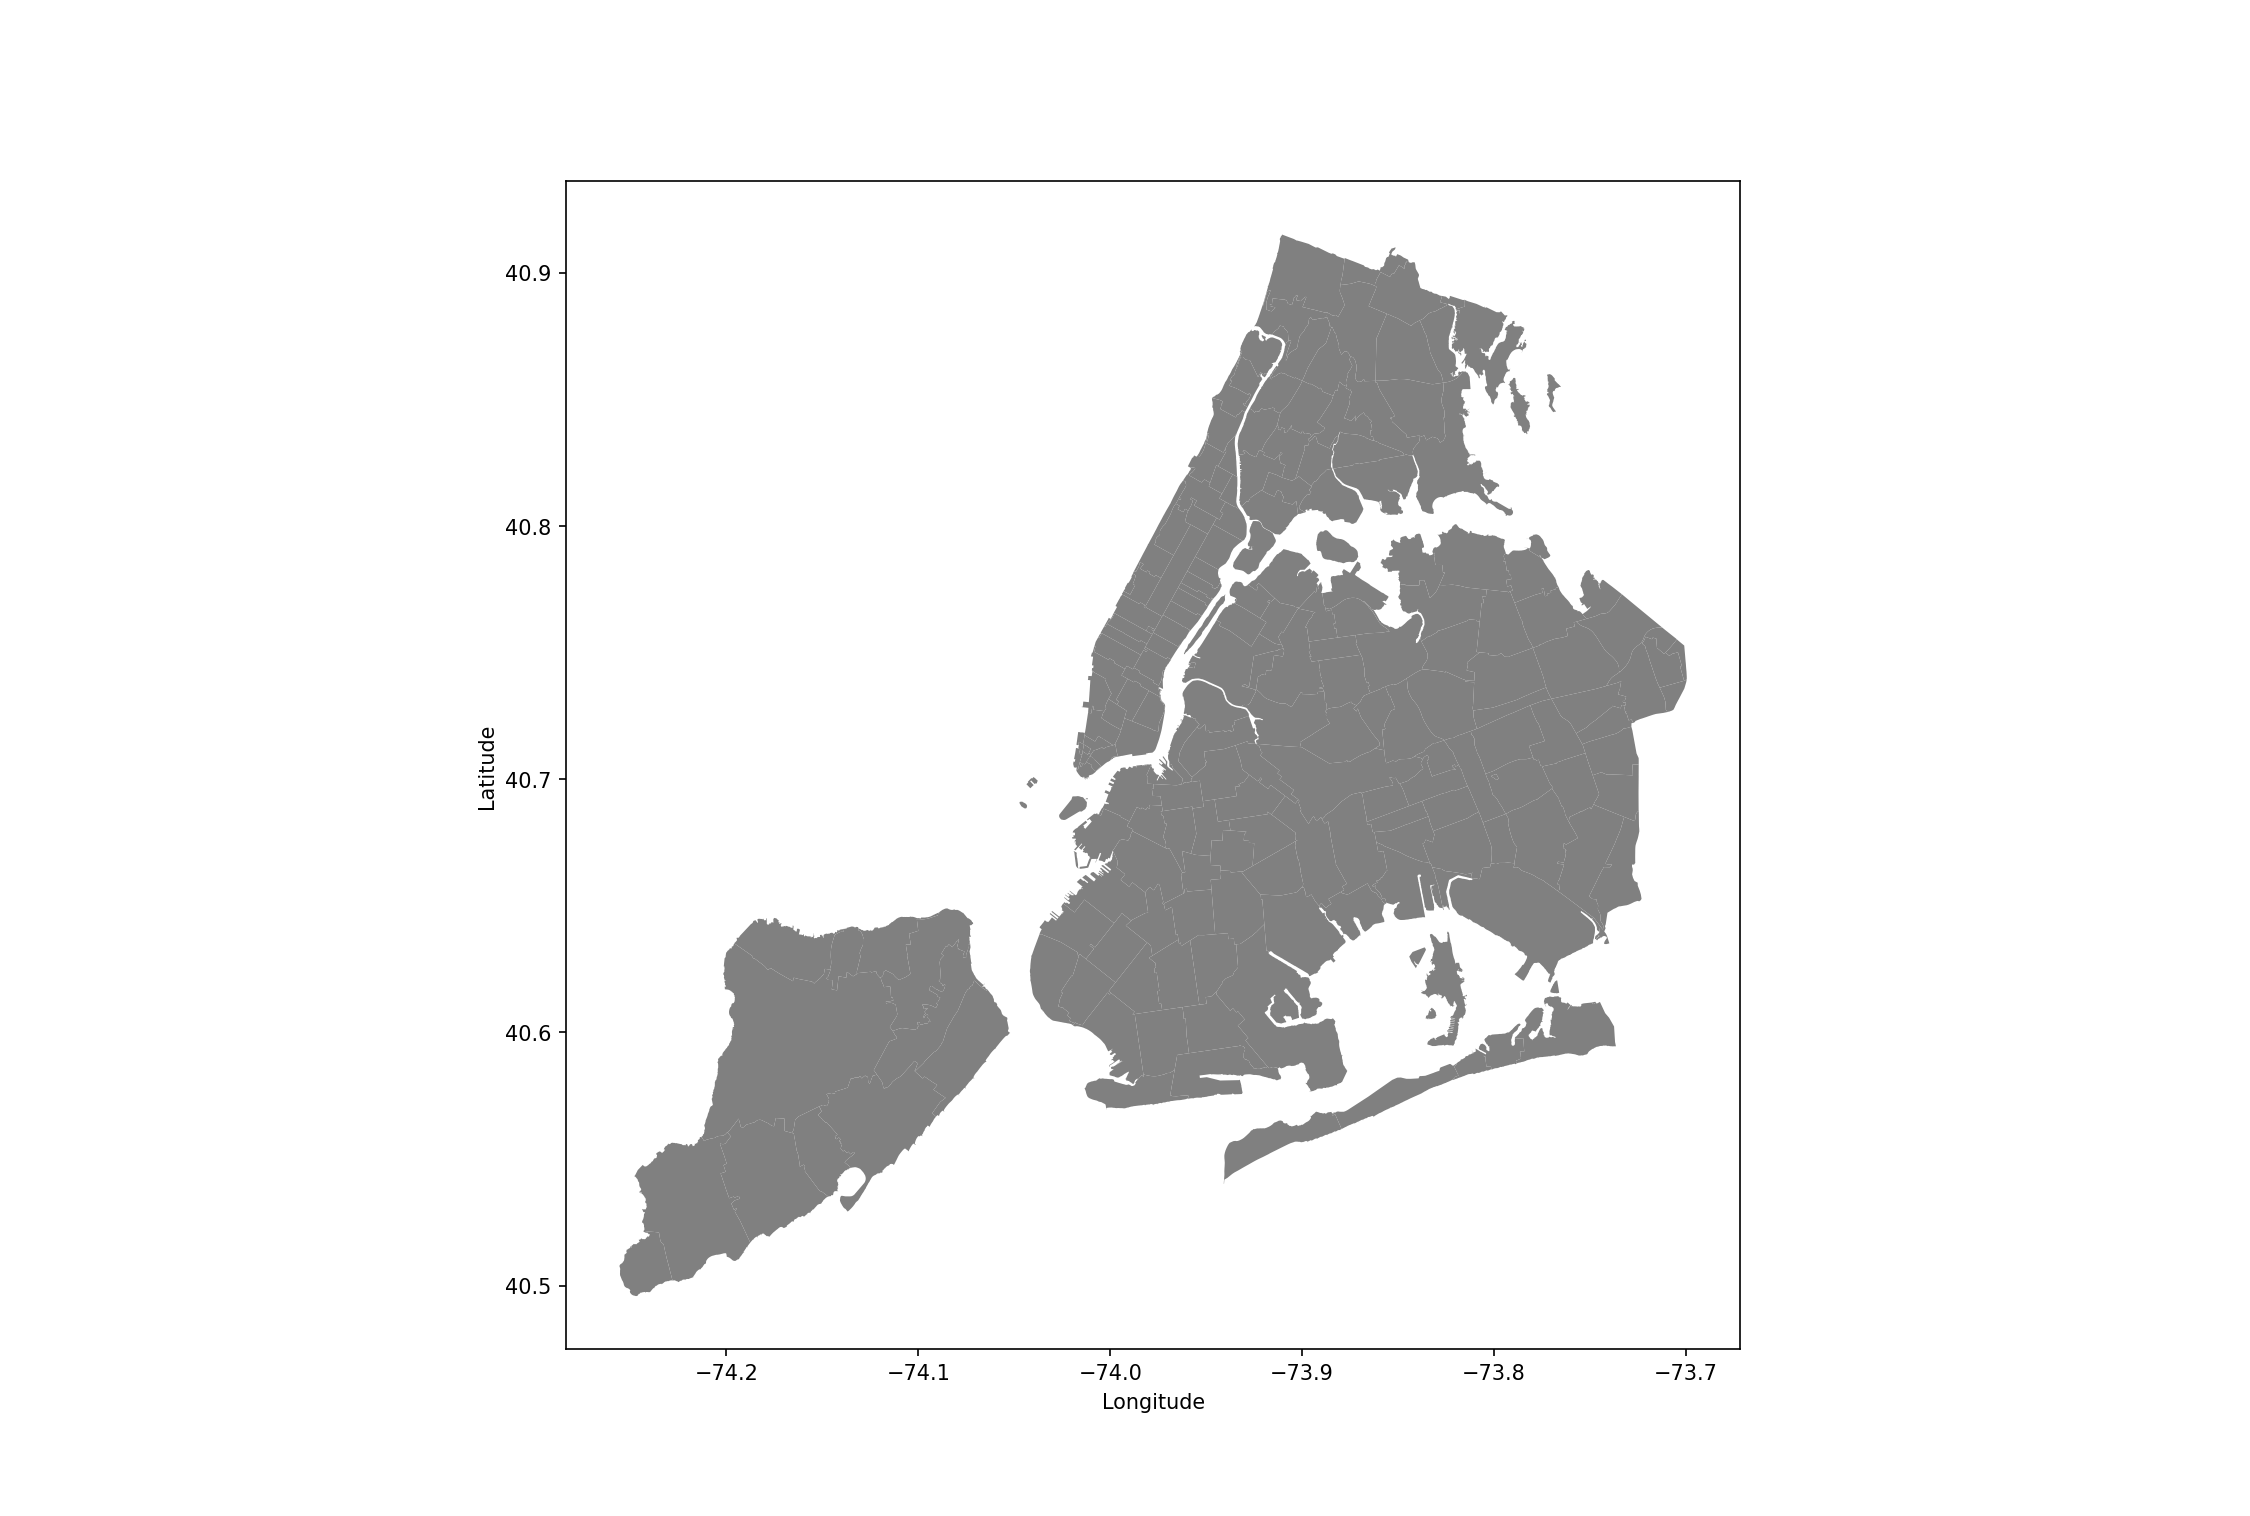
\includegraphics[trim={50 40 50 80}, clip, width=.9\linewidth,keepaspectratio]{plots/probing_outliers/3_geodata/NYCmap.png}
\caption{New York City map with zip code areas from NYC Open Data.}\label{NYCmap}
\end{center}
\end{figure}

\vspace*{-20pt}

\begin{figure}[H]
\centering
\begin{subfigure}{0.6\textwidth}
  \centering
  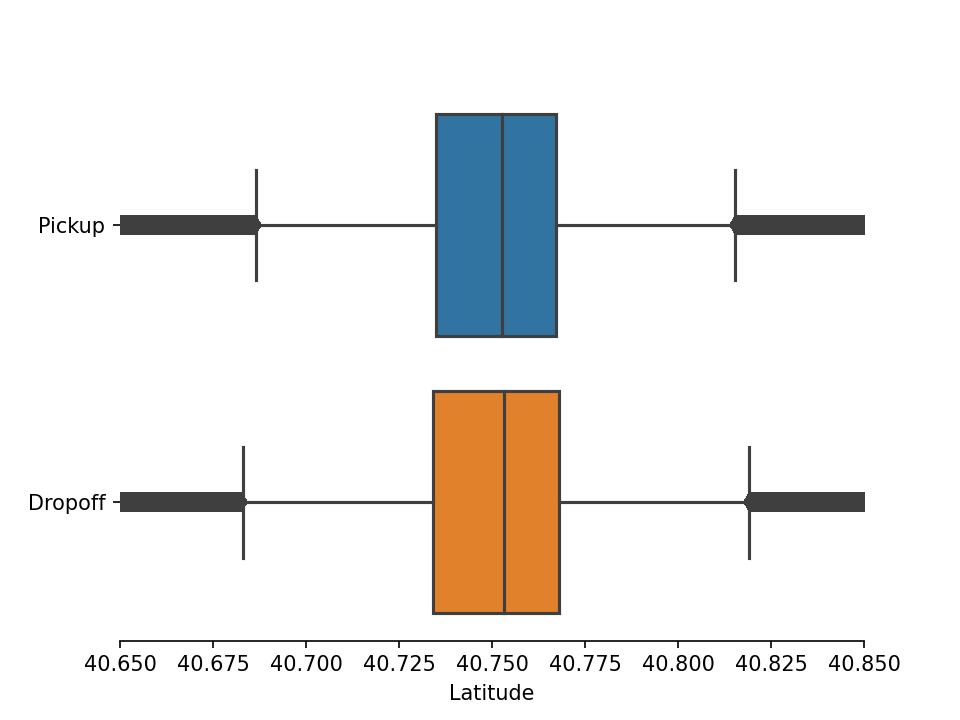
\includegraphics[width=.85\linewidth,keepaspectratio]{plots/probing_outliers/3_geodata/pickup_dropoff_latitude_training.png}
\caption{Latitudes}
\end{subfigure}% 
\hspace*{-2cm}
\begin{subfigure}{.6\textwidth}
  \centering
  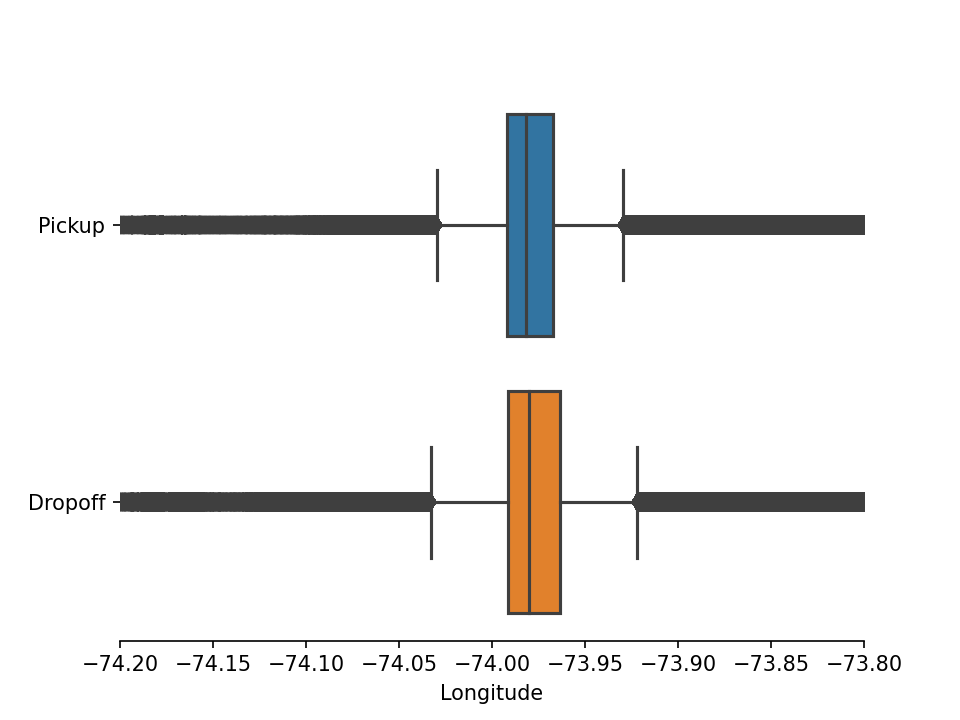
\includegraphics[width=.85\linewidth,keepaspectratio]{plots/probing_outliers/3_geodata/pickup_dropoff_longitude_training.png}
  \caption{Longitudes}
%  \label{fare_amount_2}
\end{subfigure}
\caption{Box Plots of pickup/dropoff coordinates from the thrice-truncated training set.}
\label{coordinates_box}
\end{figure}

In the next section, we will discuss how we generate new features out of the given pickup and dropoff coordinates. Among the new features obtained, here we study a) \verb|euclidean_distance_miles|: Euclidean (flat space) geodesic distance between the end point coordinates, in miles, and b) \verb|pickup_county| and \verb|dropoff_county|: the county of the pickup and dropoff points.


In \hyperref[euclidean_distance_miles_hist1]{Figure \ref*{euclidean_distance_miles_hist1}}, we plotted the Euclidean distance between the pickup and dropoff points in the \textit{thrice-truncated} training set. We observe bumps at around 60 and 75 miles respectively, on an otherwise smooth plot. There is also a much narrower bump at around 10 miles.

\begin{figure}[H]
\begin{center}
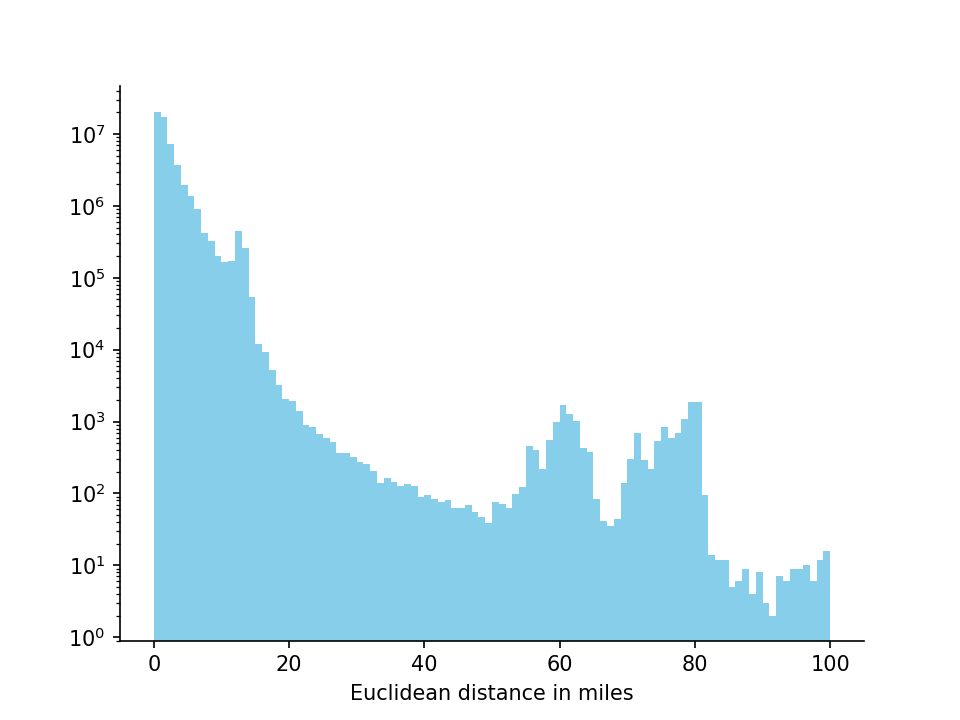
\includegraphics[width=.6\linewidth,keepaspectratio]{plots/probing_outliers/3_geodata/euclidean_distance_miles_hist.png}
\caption{Euclidean distance between pickup and dropoff points in the thrice-truncated training set.}\label{euclidean_distance_miles_hist1}
\end{center}
\end{figure}


In \hyperref[county1]{Figure \ref*{county1}}, we made a bar chart of the counties to which pickup/dropoff coordinates belong in the thrice-truncated training set. The (log) plots for the pickup and dropoff corrdinates look roughly the same, with New York county (Manhattan) having the highest counts.

\begin{figure}[H]
\centering
\begin{subfigure}{0.6\textwidth}
  \centering
  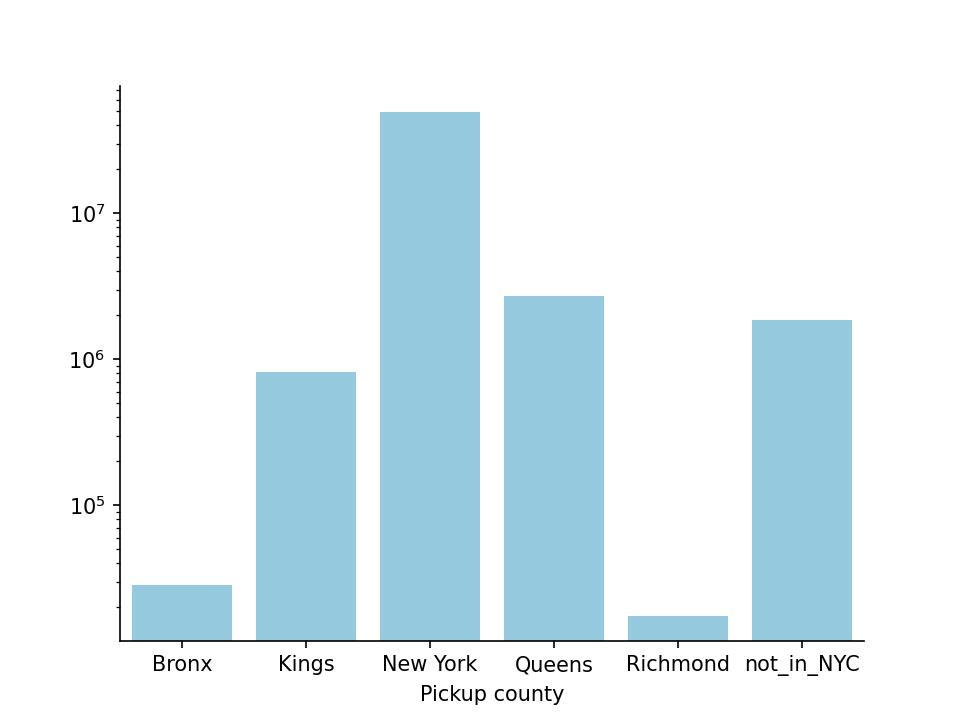
\includegraphics[width=.8\linewidth,keepaspectratio]{plots/probing_outliers/3_geodata/pickup_county_count_training.png}
\caption{Pickup}
\end{subfigure}% 
\hspace*{-2cm}
\begin{subfigure}{.6\textwidth}
  \centering
  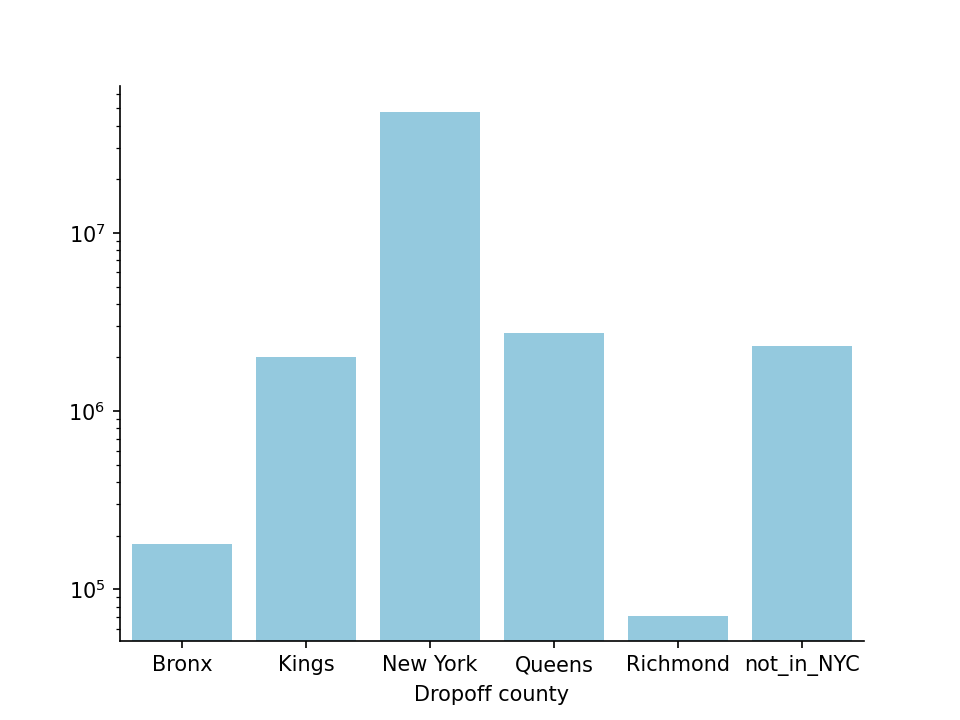
\includegraphics[width=.8\linewidth,keepaspectratio]{plots/probing_outliers/3_geodata/dropoff_county_count.png}
  \caption{Dropoff}
%  \label{fare_amount_2}
\end{subfigure}
\caption{Counties to which pickup/dropoff coordinates belong in the thrice-truncated training set.}
\label{county1}
\end{figure}

Informed by \hyperref[coordinates_box]{Figure \ref*{coordinates_box}}, we make the final truncation of the training dataset: only keep instances with latitude between 40.40 and 41.06, and longitude between -75.00 and -73.33.

\subsection{Discarding Outliers}\label{outliersec}

In summary, we have performed four truncations on the training set, keeping only the instances with
\begin{enumerate}
\item $\$2.50\leq $\verb|fare_amout| $\leq \$800$
\item $1\leq $ \verb|passenger_count| $\leq 6$
\item \verb|year| $\geq 2009$
\item $40.40 \leq $ latitudes $\leq 41.06$, $-75.00\leq$ longitudes $\leq -73.33$.
\end{enumerate}

After all these truncations, we redo some of the figures plotted above. Any previous plots (with partial truncations) not discussed in this subsection are qualitatively the same as before the \textit{full} truncation. The main differences lie in the plots about geographical data. 


In \hyperref[coordinates2]{Figure \ref*{coordinates2}}, we made the histograms of the pickup and dropoff coordinates, of the truncated training set and the test set. First, the test and training sets follow roughly the same distribution. Second, we notice slight peaks at latitude $\approx 40.65$, and at longitudes $\approx -73.8, -74.2$. Incidentally, these are roughly the coordinates of the three airports in the greater New York area\footnote{Coordinates of the airports in the greater New York area are roughly: EWR: (40.68, -74.175), JFK: (40.64, -73.78), LGA: (40.77, -73.87).}.


The Euclidean distance plot of \hyperref[euclidean_distance_miles_hist1]{Figure \ref*{euclidean_distance_miles_hist1}} now becomes \hyperref[euclidean_distance_miles_hist2]{Figure \ref*{euclidean_distance_miles_hist2}}, in which we  also plotted the test set data. Again, the  two datasets give similar behaviour. The bumps at around 60 and 75 miles we previously observed were also gone, which makes sense because, as we remarked in the beginning, the farthest driving distance within NYC is only about 45 miles. The much narrower and smaller peak at around 10 miles is still present; the \textit{driving} distance between the airports and Manhattan is about 10-15 miles.

\begin{figure}[H]
\centering
\begin{subfigure}{0.51\textwidth}
  \centering
  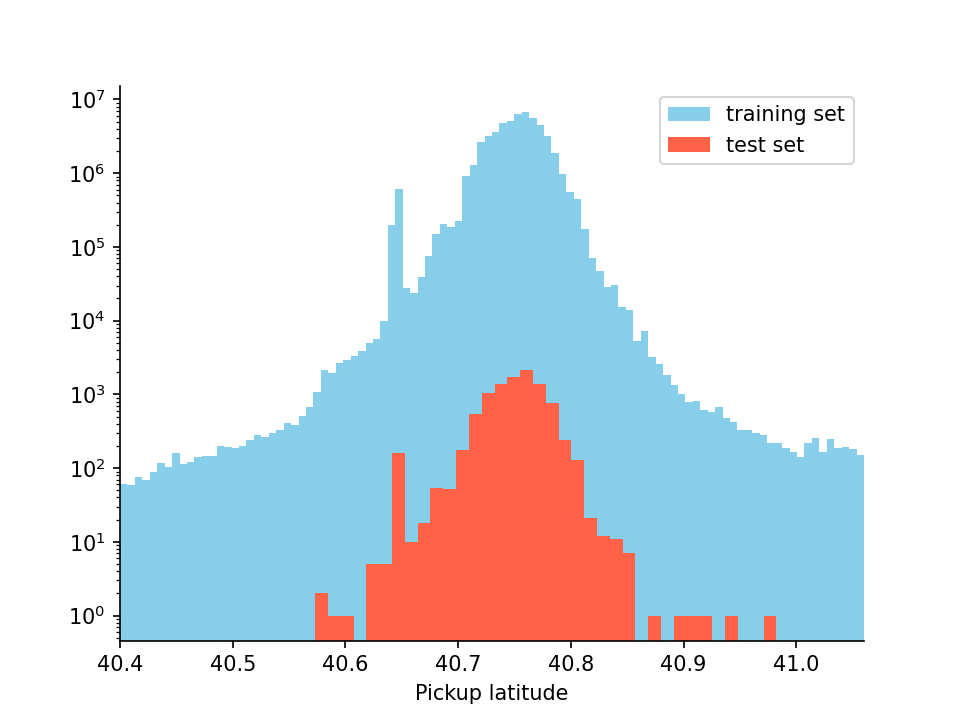
\includegraphics[width=.85\linewidth,keepaspectratio]{plots/dropped_outliers/pickup_latitude_training.png}
\caption{Pickup latitudes}
\end{subfigure}% 
\hspace*{-2cm}
\begin{subfigure}{.51\textwidth}
  \centering
  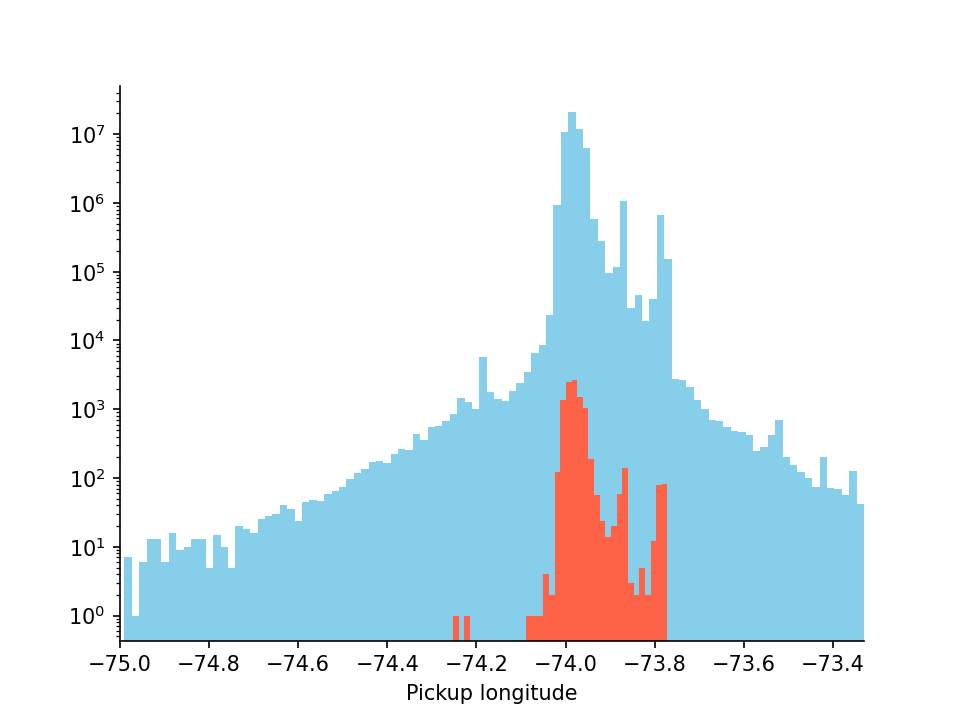
\includegraphics[width=.85\linewidth,keepaspectratio]{plots/dropped_outliers/pickup_longitude_training.png}
  \caption{Pickup longitudes}
%  \label{fare_amount_2}
\end{subfigure}
\linebreak
\begin{subfigure}{0.51\textwidth}
  \centering
  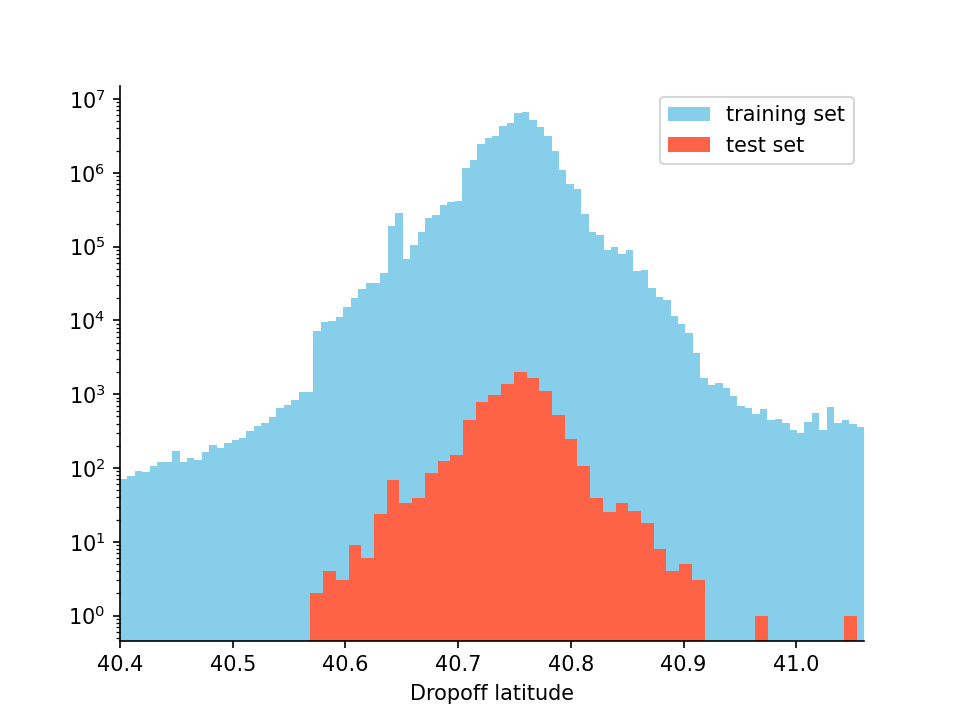
\includegraphics[width=.85\linewidth,keepaspectratio]{plots/dropped_outliers/dropoff_latitude_training.png}
\caption{Dropoff latitudes}
\end{subfigure}% 
\hspace*{-2cm}
\begin{subfigure}{.51\textwidth}
  \centering
  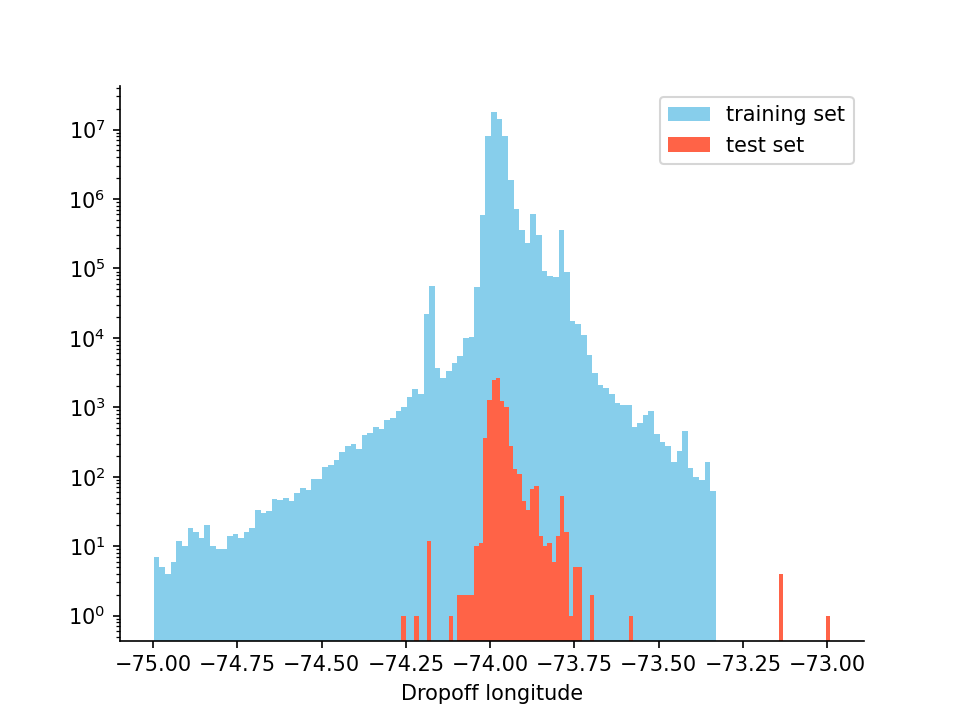
\includegraphics[width=.85\linewidth,keepaspectratio]{plots/dropped_outliers/dropoff_longitude_training.png}
  \caption{Dropoff longitudes}
%  \label{fare_amount_2}
\end{subfigure}
\caption{Pickup/dropoff coordinate histograms from the fully truncated training set and the test set.}
\label{coordinates2}
\end{figure}

\vspace*{-20pt}

\begin{figure}[H]
\begin{center}
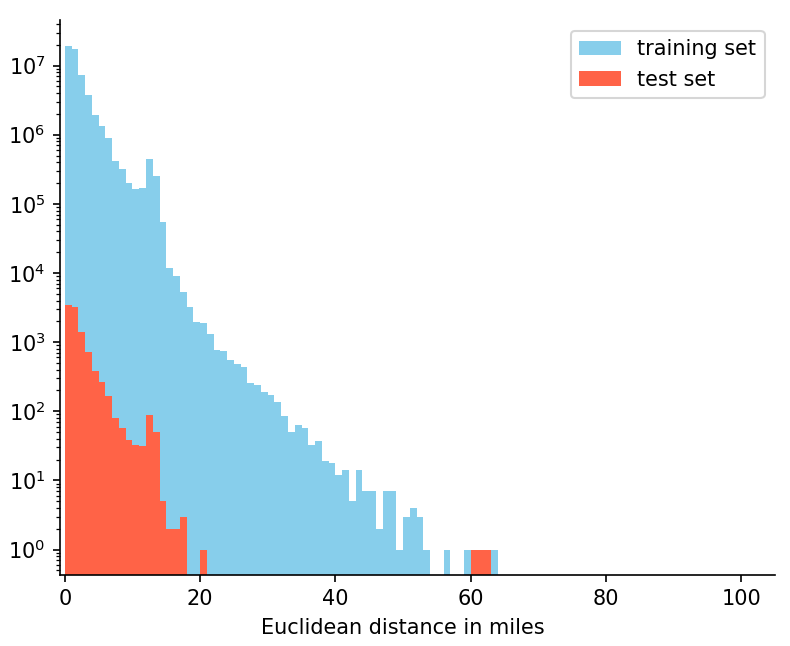
\includegraphics[width=.55\linewidth,keepaspectratio]{plots/dropped_outliers/euclidean_distance_miles_hist.png}
\caption{Euclidean distance between pickup and dropoff points from the fully truncated training set and the test set.}\label{euclidean_distance_miles_hist2}
\end{center}
\end{figure}

All in all, our training and test datasets have similar statistics. 

\subsection{Correlation Matrix}

Lastly, we plot the correlation matrix of the fully truncated training set for a select few features (due to limited space). Expectedly, the the target \verb|fare_amount| is strongly correlated with \verb|euclidean_distance_miles|, and also with the coordinates.

\begin{figure}[H]
\begin{center}
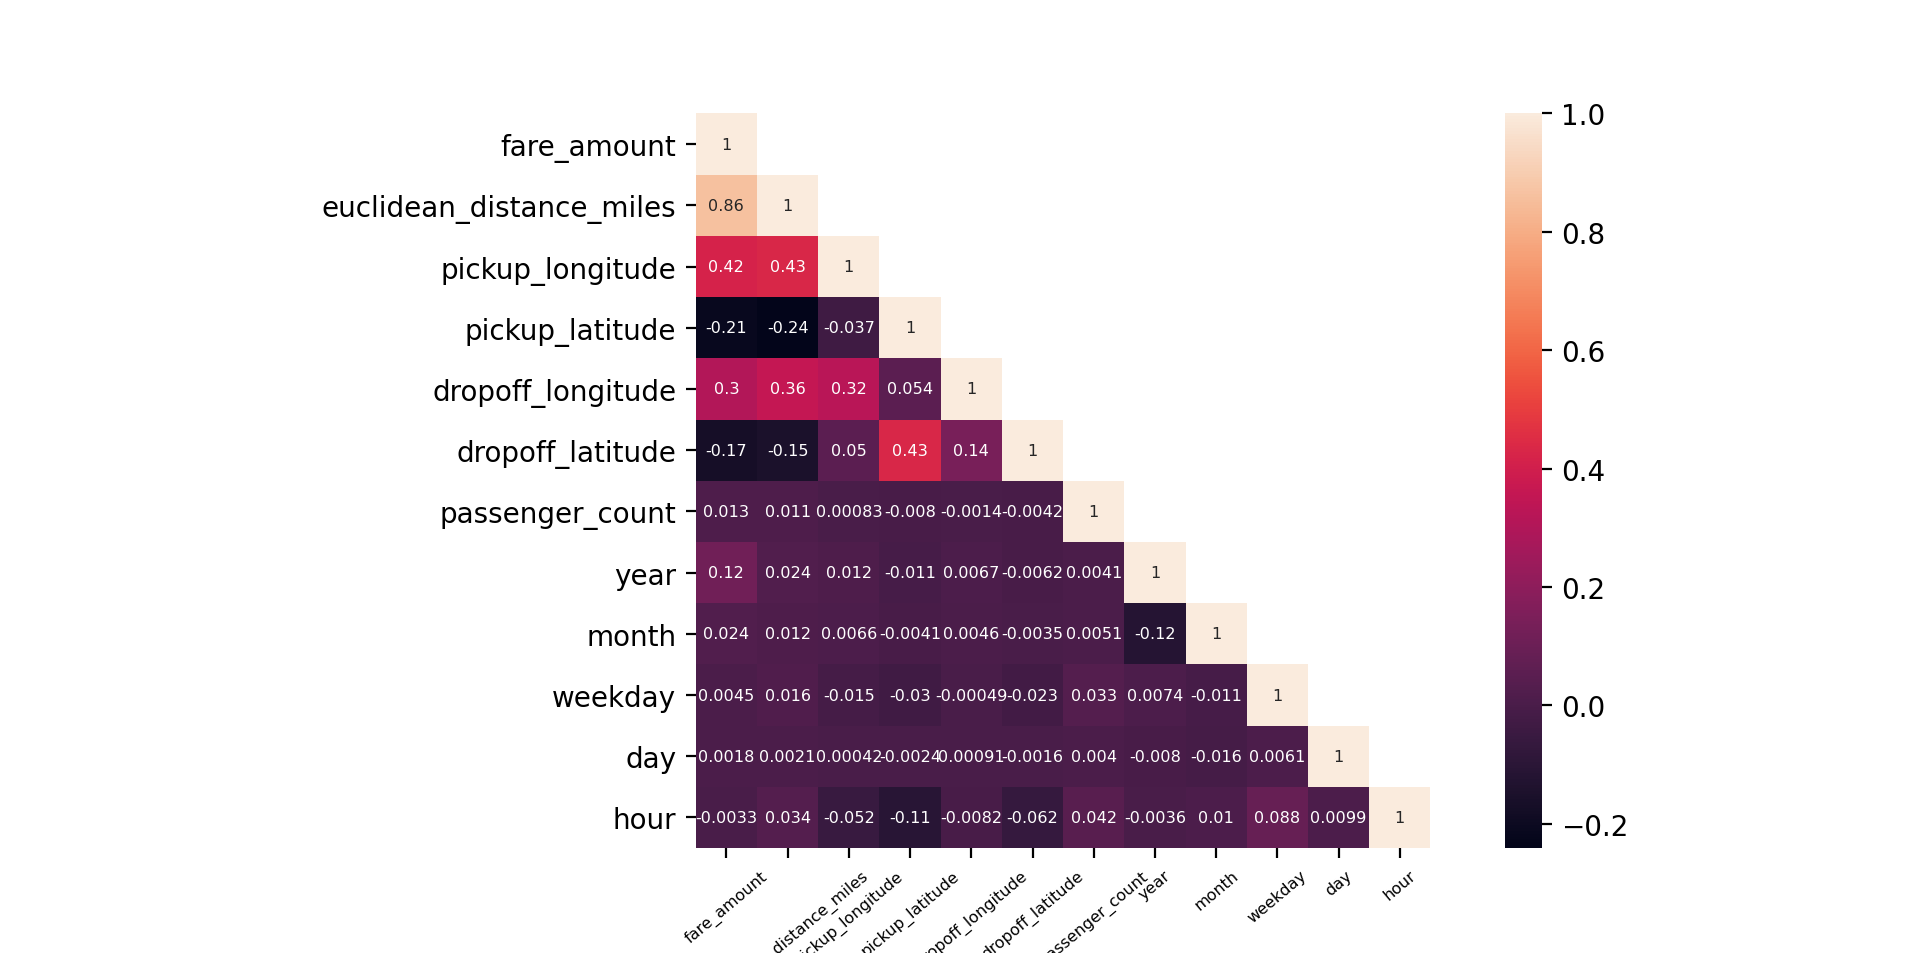
\includegraphics[width=1.1\linewidth,keepaspectratio]{plots/correlation_matrix.png}
\caption{Correlation matrix from the fully truncated training.}\label{corrmatrix}
\end{center}
\end{figure}

\section{Feature Pre-processing and Engineering}

We now describe the feature pre-processing and engineering procedure, implemented in \verb|pre-processing.py|.

\subsection{Workflow}

We first describe our workflow, where the starting point is the datetime-processed training set.

\begin{enumerate}
\item Load datetime-processed training set containing \verb|year|, \verb|month|, \verb|weekday|, \verb|day|, \verb|hour| extracted from parsed datetime
\item Diacard outliers according to \hyperref[outliersec]{Section \ref*{outliersec}}
\item Separate features and labels
\item Train-validation split: we use a 99.5-0.5 split; the validation set has $\sim$270k instances
\item Compute Euclidean distances and bearings
\item Reverse geocoding: Extract zip codes and boroughs from the coordinates, and identify which coordinates fall in the neighbourhoods of the 3 airports
\item Encoding categorical variables
\item Select feature
\item Repeat Steps 5-8 for the datetime-processed test set.
\end{enumerate}

Note that we do not perform a feature rescaling, because a) the training set is too large, and b) we anticipate using tree-based models which do not require such rescaling.

\subsection{Euclidean Distances and Bearings}

Throughout this work, we do not compute the \textit{driving} distances from the coordinates. This can actually be done with the use of the \verb|osmnx| and \verb|networkx| packages (and included in \\\verb|pre-processing.py|). We did not implement it simply due to the slow speed, considering the large size of our datasets. 

We compute the Euclidean geodesic distances and the latitudinal/longitudinal displacements instead; within the city, it is very much the same as the Haversine distances. It is computed using simple trigonometry (remembering to convert degree to radian). The bearings are computed using \verb|np.arctan2|, from which we extract its sines and cosines as features; the latter are periodic which make for better features.

\subsection{Reverse Geocoding}

By reverse geocoding, we specifically mean extracting the zip codes and boroughs (counties) from the coordinates. To this end, we import the ``ZIP Code Tabulation Areas" dataset from the US Census Gazateer which contains zip code coordinates in the US, and a dataset from NYC Open Data that contains a map from NYC zip codes to counties. These two datasets are first merged. Then, using \verb|sklearn.neighbors.KDTree| for its high speed, we extract the zip codes and counties from the coordinates. Furthermore, from this we also identify instances which begin/end at the neighbourhoods (taking into account the non-exactness of \verb|KDTree|) of one of the airports, as well as those which begin and end in the same county.

All in all, the geographical new features are \verb|pickup_zipcode|, \verb|pickup_county|, \\\verb|dropoff_zipcode|, \verb|dropoff_county|, \verb|pickup_airport|, \verb|pickup_airport| \\and \verb|dropoff_pickup_same_county|. The latter three are Boolean.

\subsection{Encoding Categorical Variables}
At this point we have the following categorical variables: \verb|passenger_count|, \verb|pickup_county|, \verb|dropoff_county|, \verb|weekday|, \verb|year|, \verb|month|, \verb|day|, \verb|hour|, \verb|pickup_zipcode| and \verb|dropoff_zipcode|. Inspired by the analysis from the last section, we perform one-hot encoding on \verb|passenger_count|, \verb|pickup_county| and \verb|dropoff_county|, frequency encoding on \verb|weekday| using \verb|category_encoders|, and (target) mean encoding on \verb|year|, \verb|month|, \verb|day|, \verb|hour|, \verb|pickup_zipcode| and \verb|dropoff_zipcode|.

\subsection{Feature Selection}

We select the following features: 

\begin{lstlisting}[language=Python, basicstyle=\footnotesize]
['pickup_longitude', 'pickup_latitude', 'dropoff_longitude',
'dropoff_latitude', 'daylight_saving', 'long_displacement',
'lat_displacement', 'euclidean_distance_miles', 
'sin_direction', 'cos_direction', 'dropoff_pickup_same_county',
'pickup_airport', 'dropoff_airport', 'passenger_count_1',
'passenger_count_2', 'passenger_count_3', 'passenger_count_4',
'passenger_count_5', 'passenger_count_6', 'pickup_county_Bronx',
'pickup_county_Kings', 'pickup_county_New York', 'pickup_county_Queens',
'pickup_county_Richmond', 'pickup_county_not_in_NYC',
'dropoff_county_Bronx', 'dropoff_county_Kings',
'dropoff_county_New York', 'dropoff_county_Queens',
'dropoff_county_Richmond', 'dropoff_county_not_in_NYC',
'weekday_freq_encoded', 'year_mean_encoded', 'month_mean_encoded',
'day_mean_encoded', 'hour_mean_encoded', 'pickup_zipcode_mean_encoded',
'dropoff_zipcode_mean_encoded']
\end{lstlisting}

Lastly, we downcast some of the features where appropriate.

\section{Models}

Given the large size of the training set, we use \verb|xgboost.XGBRegressor| and \verb|lightgbm.LGBMRegressor|, hoping that everything can fit into the 16GB RAM of the local machine. It turns out it cannot. As a compromise, we only use part of the training (the ``train" after the train-validation split) set to train the models. In principle, we should select the best model based on the lowest validation RMSE. But given the nature of Kaggle competition, we simply training them and submit all the predictions.

\verb|xgboost.XGBRegressor| turns out to be more resource-hungry. We use 5 million instances from the training set, with the following hyperparameters:
\begin{lstlisting}[language=Python, basicstyle=\footnotesize]
XGBR_model = XGBRegressor(eval_metric = "rmse", 
                          learning_rate = 0.05, 
                          max_depth = 8,
                          n_estimators = 100,
                          reg_lambda = 0.7,
                          n_jobs = 6)
\end{lstlisting}
This results in an RMSE of 3.22539 on the test set, as verified by submitting to Kaggle. 


For \verb|lightgbm.LGBMRegressor| we use the following hyperparameters
\begin{lstlisting}[language=Python, basicstyle=\footnotesize]
LGBMreg = lightgbm.LGBMRegressor(boosting_type = 'gbdt', 
                            learning_rate = 0.02, 
                            num_leaves = 800,
                            n_estimators = 500, 
                            num_iterations = 5000, 
                            max_bin = 500, 
                            feature_fraction = 0.7, 
                            bagging_fraction = 0.7,
                            lambda_l2 = 0.5,
                            max_depth = 25,
                            silent = False)
\end{lstlisting}
With 5 million training instances, it gives an RMSE of 2.99131 on the test set, and it is significantly faster and less resource-hogging than \verb|xgboost.XGBRegressor|. (We could try to tune the hyperparameters of the latter, but the time commitment is too high.) With 20 million training instances, the RMSE improved slightly to 2.96150. Any more training instances maxed out the RAM and caused a black screen of death.

Our choices of hyperparameters were inspired by our work on a previous project, which is another \href{https://www.kaggle.com/c/nyc-taxi-trip-duration/overview}{Kaggle competition} predicting NYC taxi trip duration, given similar features as this project.

\vspace*{-12pt}

\section{Predictions}

Using \verb|lightgbm.LGBMRegressor| trained with 20 million training instances, the test set predictions take the following distribution:

\begin{figure}[H]
\begin{center}
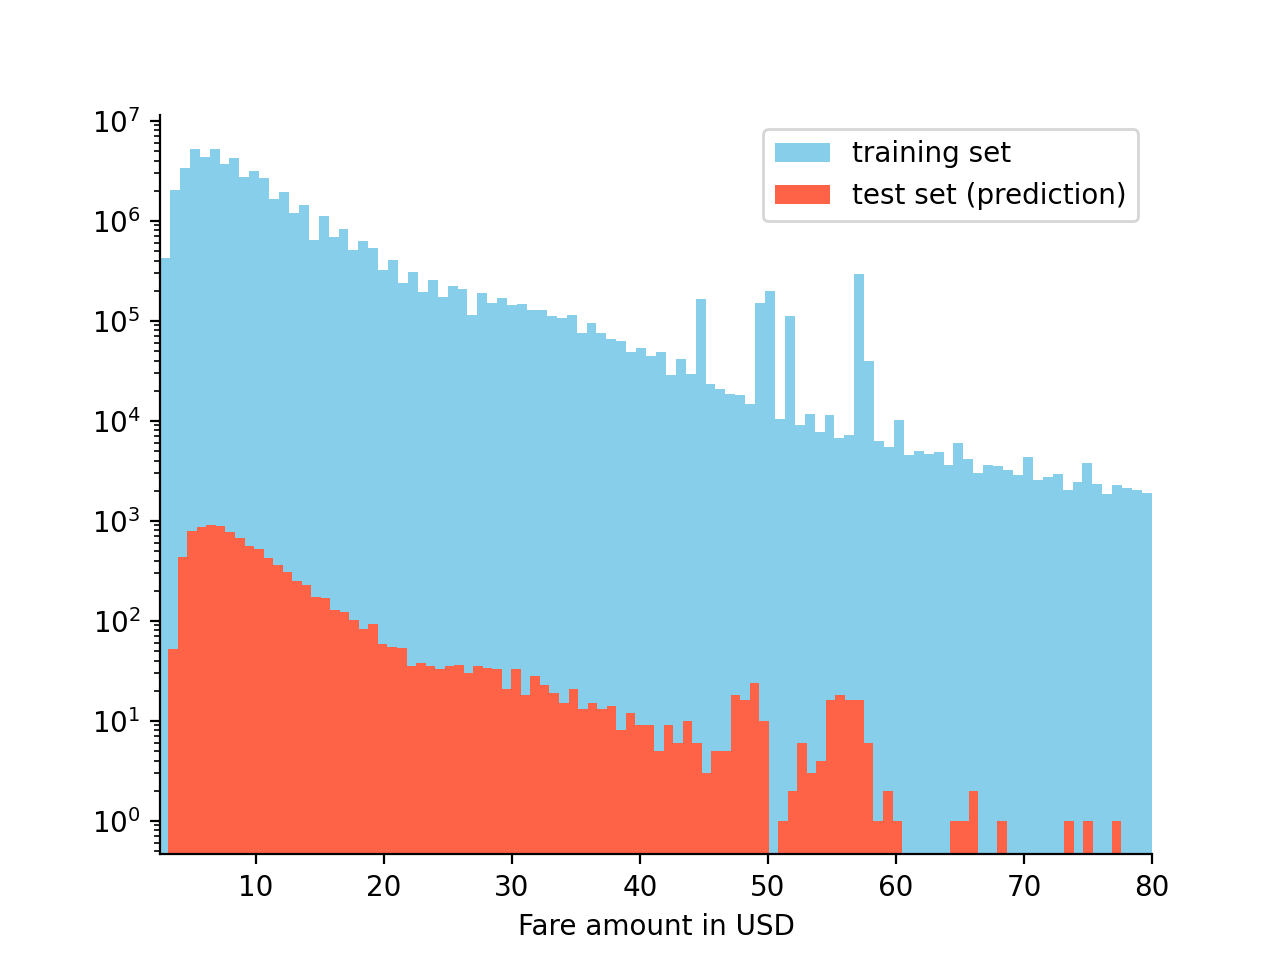
\includegraphics[trim={0 0 0 10}, clip, width=0.7\linewidth,keepaspectratio]{plots/fare_amount_trains_vs_test_predict_hist_20M_LGBM.png}
\caption{Test set predictions (red) from \texttt{lightgbm.LGBMRegressor} trained with 20 million training instances. The training set (blue) is the fully truncated set before the train-validation split.}\label{pred}
\end{center}
\end{figure}

This shows that the predictions take a very similar distribution as the full truncated training set. They both exhibit slight bumps at $\sim\$$55, which could be due to the flat rate between the airports and Manhattan.

The \texttt{lightgbm.LGBMRegressor} model gives the following feature importances:

\begin{figure}[H]
\begin{center}
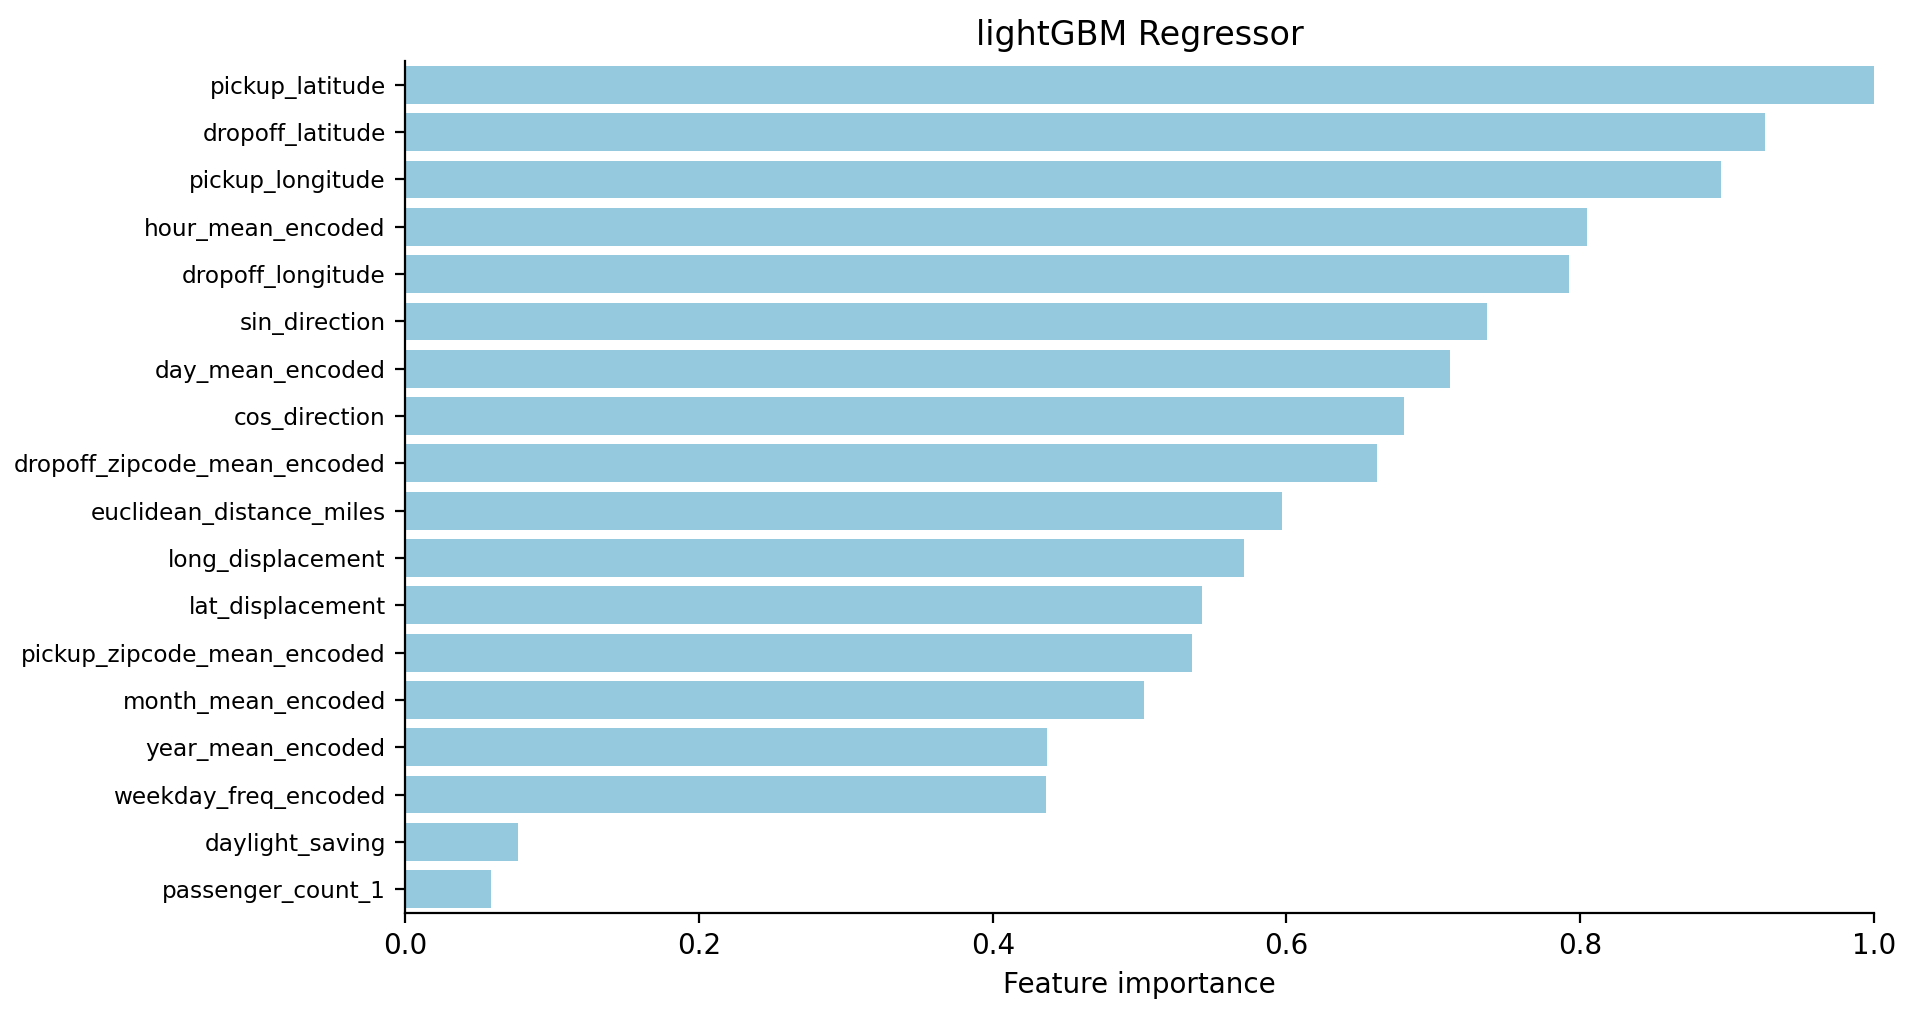
\includegraphics[width=0.9\linewidth,keepaspectratio]{plots/lightgbm_feature_importances20M.png}
\caption{Feature importances of \texttt{lightgbm.LGBMRegressor} trained with 20 million training instances, normalised to one. We discarded some features with low importances in this plot.}\label{featimp}
\end{center}
\end{figure}

This agrees with out intuition: geographical data strongly correlate with the taxi fare. The \verb|hour| of the day also ranked among the highest, which could due to the rush hour/overnight surcharges. The \verb|month|, \verb|year| and \verb|weekday| are also somewhat important, which may be due to holiday seasons, improving economy during 2009-2015, people rushing to work during the weekdays, etc.

\section{Future Work}

We have missed out a few elements that can improve our performance. First is extracting the driving distances. I am not sure how it can be done efficiently, but we can keep looking. Second, we should seek to implement \verb|dask| to use the whole training set for model training. Third, we can further tune the hyperparameters to improve model performance.


\section{Acknowledgment}

We acknowledge the authors from various sources online, whose tools and techniques were borrowed and implemented in our codes. (I didn't keep track of the references.)


%
%\renewcommand\refname{References}
%\bibliographystyle{utphys}
%\bibliography{references}
%
%\begin{filecontents}[overwrite]{references.bib}
%@article{Dymarsky:2020qom,
%    author = "Dymarsky, Anatoly and Shapere, Alfred",
%    title = "{Quantum stabilizer codes, lattices, and CFTs}",
%    eprint = "2009.01244",
%    archivePrefix = "arXiv",
%    primaryClass = "hep-th",
%    doi = "10.1007/JHEP03(2021)160",
%    journal = "JHEP",
%    volume = "21",
%    pages = "160",
%    year = "2020"
%}
%
%@book{Zwillinger,
%  author    = {Zwillinger, D.}, 
%  title     = {Standard Mathematical Tables and Formulae},
%  publisher = {Academic Press},
%  year      = 2003,
%  edition   = 8,
%  isbn      = {978-0-12-384933-5}
%}
%
%
%\end{filecontents}


\end{document}

